\documentclass[11pt]{article}

% Shared notes settings for Applied Machine Learning lectures (UPES).
% Keep this file free of \documentclass to allow reuse via \input.

\usepackage[utf8]{inputenc}
\usepackage[T1]{fontenc}
\usepackage{lmodern}          % scalable T1 fonts; without this pdflatex falls back
\input{glyphtounicode}        % to bitmapped EC Type 3 and the PDFs are neither
\pdfgentounicode=1            % searchable nor screen-reader friendly
\usepackage[a4paper,margin=1in]{geometry}
\usepackage{hyperref}
\usepackage{xurl}
\usepackage{booktabs}
\usepackage{amsmath}
\usepackage{amssymb}
\usepackage{listings}
\usepackage{xcolor}
\usepackage{enumitem}
\usepackage{parskip}

% Code listings (Python-oriented for this subject).
\lstset{
  language=Python,
  basicstyle=\ttfamily\small,
  keywordstyle=\color{blue},
  commentstyle=\color{gray},
  stringstyle=\color{teal},
  showstringspaces=false,
  columns=fullflexible,
  frame=single,
  framerule=0.2pt,
  breaklines=true
}

\setlist[itemize]{topsep=0.3em,itemsep=0.2em}
\setlist[enumerate]{topsep=0.3em,itemsep=0.2em}

% Simple per-section source line.
\newcommand{\notesources}[1]{\par\noindent{\small\color{gray}\textit{Sources:} \sloppy #1\par}}

% Unit-wise source strings for this subject (used by slides + notes).
% Path is relative to the lecture `latex/` folder (the compilation CWD).
\IfFileExists{../../../_shared/aml-sources.tex}{%
  % Source strings for Applied Machine Learning (CSAI2017P) — used by slides + notes.
% Prescribed texts and reference books are taken from the course syllabus.
% Support texts are the author-hosted open-access editions:
%   statlearning.com            (ISL with Python)
%   probml.github.io/pml-book   (Murphy, Probabilistic Machine Learning)
%   d2l.ai                      (Dive into Deep Learning)
%   mml-book.github.io          (Mathematics for Machine Learning)

\newcommand{\AMLRepoURL}{https://github.com/tali7c/Applied-Machine-Learning}

% --- prescribed -------------------------------------------------------------
\newcommand{\AMLPrescribed}{%
M\"uller and Guido, \textit{Introduction to Machine Learning with Python}, O'Reilly, 2016.;%
Bishop, \textit{Pattern Recognition and Machine Learning}, Springer, 2006.;%
Murphy, \textit{Machine Learning: A Probabilistic Perspective}, MIT Press, 2012.;%
Han, Kamber and Pei, \textit{Data Mining: Concepts and Techniques} (3e), Morgan Kaufmann, 2012.%
}

% --- unit-wise ---------------------------------------------------------------
\newcommand{\AMLUnitISources}{%
M\"uller and Guido, \textit{Introduction to Machine Learning with Python}, Ch. 1.;%
Bishop, \textit{Pattern Recognition and Machine Learning}, Ch. 1.;%
Murphy, \textit{Probabilistic Machine Learning: An Introduction}, MIT Press, 2022, Ch. 1.;%
Mitchell, \textit{Machine Learning}, McGraw Hill, 1997, Ch. 1.;%
Scikit-learn documentation, accessed 2026-08-04.%
}

\newcommand{\AMLUnitIISources}{%
Bishop, \textit{Pattern Recognition and Machine Learning}, \S1.5, \S4.3, \S7.1.;%
Zhang, Lipton, Li and Smola, \textit{Dive into Deep Learning}, \S3.4.;%
Shalev-Shwartz and Ben-David, \textit{Understanding Machine Learning}, Ch. 15.;%
Murphy, \textit{Probabilistic Machine Learning: An Introduction}, Ch. 5.%
}

\newcommand{\AMLUnitIIISources}{%
Zhang, Lipton, Li and Smola, \textit{Dive into Deep Learning}, Ch. 12 (Optimization Algorithms).;%
Deisenroth, Faisal and Ong, \textit{Mathematics for Machine Learning}, Ch. 7.;%
Kingma and Ba, ``Adam: A Method for Stochastic Optimization,'' ICLR 2015.;%
Ruder, ``An overview of gradient descent optimization algorithms,'' arXiv:1609.04747, 2016.%
}

\newcommand{\AMLUnitIVSources}{%
Han, Kamber and Pei, \textit{Data Mining: Concepts and Techniques} (3e), Ch. 3.;%
M\"uller and Guido, \textit{Introduction to Machine Learning with Python}, Ch. 3--4.;%
James, Witten, Hastie, Tibshirani and Taylor, \textit{An Introduction to Statistical Learning with Python}, Ch. 5--6, 12.;%
Scikit-learn documentation (preprocessing, model selection), accessed 2026-08-04.%
}

\newcommand{\AMLUnitVSources}{%
James et al., \textit{An Introduction to Statistical Learning with Python}, Ch. 3--6.;%
Bishop, \textit{Pattern Recognition and Machine Learning}, Ch. 3.;%
Deisenroth, Faisal and Ong, \textit{Mathematics for Machine Learning}, Ch. 9.;%
M\"uller and Guido, \textit{Introduction to Machine Learning with Python}, \S2.3.%
}

\newcommand{\AMLUnitVISources}{%
Han, Kamber and Pei, \textit{Data Mining: Concepts and Techniques} (3e), Ch. 8--9.;%
James et al., \textit{An Introduction to Statistical Learning with Python}, Ch. 8--9.;%
Bishop, \textit{Pattern Recognition and Machine Learning}, Ch. 4--5, 7, 14.;%
Zhang et al., \textit{Dive into Deep Learning}, Ch. 5.%
}

\newcommand{\AMLUnitVIISources}{%
Han, Kamber and Pei, \textit{Data Mining: Concepts and Techniques} (3e), Ch. 10.;%
James et al., \textit{An Introduction to Statistical Learning with Python}, Ch. 12.;%
M\"uller and Guido, \textit{Introduction to Machine Learning with Python}, \S3.5.;%
Ester, Kriegel, Sander and Xu, ``A density-based algorithm for discovering clusters (DBSCAN),'' KDD 1996.%
}

\newcommand{\AMLLabSources}{%
M\"uller and Guido, \textit{Introduction to Machine Learning with Python}, companion notebooks.;%
McKinney, \textit{Python for Data Analysis} (3e), O'Reilly, 2022.;%
Scikit-learn user guide, accessed 2026-08-04.;%
Matplotlib and Seaborn documentation, accessed 2026-08-04.%
}
%
}{%
  % Faculty copies live under `private/` so their compile CWD is different.
  \IfFileExists{../../../../public/_shared/aml-sources.tex}{%
    % Source strings for Applied Machine Learning (CSAI2017P) — used by slides + notes.
% Prescribed texts and reference books are taken from the course syllabus.
% Support texts are the author-hosted open-access editions:
%   statlearning.com            (ISL with Python)
%   probml.github.io/pml-book   (Murphy, Probabilistic Machine Learning)
%   d2l.ai                      (Dive into Deep Learning)
%   mml-book.github.io          (Mathematics for Machine Learning)

\newcommand{\AMLRepoURL}{https://github.com/tali7c/Applied-Machine-Learning}

% --- prescribed -------------------------------------------------------------
\newcommand{\AMLPrescribed}{%
M\"uller and Guido, \textit{Introduction to Machine Learning with Python}, O'Reilly, 2016.;%
Bishop, \textit{Pattern Recognition and Machine Learning}, Springer, 2006.;%
Murphy, \textit{Machine Learning: A Probabilistic Perspective}, MIT Press, 2012.;%
Han, Kamber and Pei, \textit{Data Mining: Concepts and Techniques} (3e), Morgan Kaufmann, 2012.%
}

% --- unit-wise ---------------------------------------------------------------
\newcommand{\AMLUnitISources}{%
M\"uller and Guido, \textit{Introduction to Machine Learning with Python}, Ch. 1.;%
Bishop, \textit{Pattern Recognition and Machine Learning}, Ch. 1.;%
Murphy, \textit{Probabilistic Machine Learning: An Introduction}, MIT Press, 2022, Ch. 1.;%
Mitchell, \textit{Machine Learning}, McGraw Hill, 1997, Ch. 1.;%
Scikit-learn documentation, accessed 2026-08-04.%
}

\newcommand{\AMLUnitIISources}{%
Bishop, \textit{Pattern Recognition and Machine Learning}, \S1.5, \S4.3, \S7.1.;%
Zhang, Lipton, Li and Smola, \textit{Dive into Deep Learning}, \S3.4.;%
Shalev-Shwartz and Ben-David, \textit{Understanding Machine Learning}, Ch. 15.;%
Murphy, \textit{Probabilistic Machine Learning: An Introduction}, Ch. 5.%
}

\newcommand{\AMLUnitIIISources}{%
Zhang, Lipton, Li and Smola, \textit{Dive into Deep Learning}, Ch. 12 (Optimization Algorithms).;%
Deisenroth, Faisal and Ong, \textit{Mathematics for Machine Learning}, Ch. 7.;%
Kingma and Ba, ``Adam: A Method for Stochastic Optimization,'' ICLR 2015.;%
Ruder, ``An overview of gradient descent optimization algorithms,'' arXiv:1609.04747, 2016.%
}

\newcommand{\AMLUnitIVSources}{%
Han, Kamber and Pei, \textit{Data Mining: Concepts and Techniques} (3e), Ch. 3.;%
M\"uller and Guido, \textit{Introduction to Machine Learning with Python}, Ch. 3--4.;%
James, Witten, Hastie, Tibshirani and Taylor, \textit{An Introduction to Statistical Learning with Python}, Ch. 5--6, 12.;%
Scikit-learn documentation (preprocessing, model selection), accessed 2026-08-04.%
}

\newcommand{\AMLUnitVSources}{%
James et al., \textit{An Introduction to Statistical Learning with Python}, Ch. 3--6.;%
Bishop, \textit{Pattern Recognition and Machine Learning}, Ch. 3.;%
Deisenroth, Faisal and Ong, \textit{Mathematics for Machine Learning}, Ch. 9.;%
M\"uller and Guido, \textit{Introduction to Machine Learning with Python}, \S2.3.%
}

\newcommand{\AMLUnitVISources}{%
Han, Kamber and Pei, \textit{Data Mining: Concepts and Techniques} (3e), Ch. 8--9.;%
James et al., \textit{An Introduction to Statistical Learning with Python}, Ch. 8--9.;%
Bishop, \textit{Pattern Recognition and Machine Learning}, Ch. 4--5, 7, 14.;%
Zhang et al., \textit{Dive into Deep Learning}, Ch. 5.%
}

\newcommand{\AMLUnitVIISources}{%
Han, Kamber and Pei, \textit{Data Mining: Concepts and Techniques} (3e), Ch. 10.;%
James et al., \textit{An Introduction to Statistical Learning with Python}, Ch. 12.;%
M\"uller and Guido, \textit{Introduction to Machine Learning with Python}, \S3.5.;%
Ester, Kriegel, Sander and Xu, ``A density-based algorithm for discovering clusters (DBSCAN),'' KDD 1996.%
}

\newcommand{\AMLLabSources}{%
M\"uller and Guido, \textit{Introduction to Machine Learning with Python}, companion notebooks.;%
McKinney, \textit{Python for Data Analysis} (3e), O'Reilly, 2022.;%
Scikit-learn user guide, accessed 2026-08-04.;%
Matplotlib and Seaborn documentation, accessed 2026-08-04.%
}
%
  }{%
    % Question papers live at `private/<family>/<instrument>/`.
    \IfFileExists{../../../public/_shared/aml-sources.tex}{%
      % Source strings for Applied Machine Learning (CSAI2017P) — used by slides + notes.
% Prescribed texts and reference books are taken from the course syllabus.
% Support texts are the author-hosted open-access editions:
%   statlearning.com            (ISL with Python)
%   probml.github.io/pml-book   (Murphy, Probabilistic Machine Learning)
%   d2l.ai                      (Dive into Deep Learning)
%   mml-book.github.io          (Mathematics for Machine Learning)

\newcommand{\AMLRepoURL}{https://github.com/tali7c/Applied-Machine-Learning}

% --- prescribed -------------------------------------------------------------
\newcommand{\AMLPrescribed}{%
M\"uller and Guido, \textit{Introduction to Machine Learning with Python}, O'Reilly, 2016.;%
Bishop, \textit{Pattern Recognition and Machine Learning}, Springer, 2006.;%
Murphy, \textit{Machine Learning: A Probabilistic Perspective}, MIT Press, 2012.;%
Han, Kamber and Pei, \textit{Data Mining: Concepts and Techniques} (3e), Morgan Kaufmann, 2012.%
}

% --- unit-wise ---------------------------------------------------------------
\newcommand{\AMLUnitISources}{%
M\"uller and Guido, \textit{Introduction to Machine Learning with Python}, Ch. 1.;%
Bishop, \textit{Pattern Recognition and Machine Learning}, Ch. 1.;%
Murphy, \textit{Probabilistic Machine Learning: An Introduction}, MIT Press, 2022, Ch. 1.;%
Mitchell, \textit{Machine Learning}, McGraw Hill, 1997, Ch. 1.;%
Scikit-learn documentation, accessed 2026-08-04.%
}

\newcommand{\AMLUnitIISources}{%
Bishop, \textit{Pattern Recognition and Machine Learning}, \S1.5, \S4.3, \S7.1.;%
Zhang, Lipton, Li and Smola, \textit{Dive into Deep Learning}, \S3.4.;%
Shalev-Shwartz and Ben-David, \textit{Understanding Machine Learning}, Ch. 15.;%
Murphy, \textit{Probabilistic Machine Learning: An Introduction}, Ch. 5.%
}

\newcommand{\AMLUnitIIISources}{%
Zhang, Lipton, Li and Smola, \textit{Dive into Deep Learning}, Ch. 12 (Optimization Algorithms).;%
Deisenroth, Faisal and Ong, \textit{Mathematics for Machine Learning}, Ch. 7.;%
Kingma and Ba, ``Adam: A Method for Stochastic Optimization,'' ICLR 2015.;%
Ruder, ``An overview of gradient descent optimization algorithms,'' arXiv:1609.04747, 2016.%
}

\newcommand{\AMLUnitIVSources}{%
Han, Kamber and Pei, \textit{Data Mining: Concepts and Techniques} (3e), Ch. 3.;%
M\"uller and Guido, \textit{Introduction to Machine Learning with Python}, Ch. 3--4.;%
James, Witten, Hastie, Tibshirani and Taylor, \textit{An Introduction to Statistical Learning with Python}, Ch. 5--6, 12.;%
Scikit-learn documentation (preprocessing, model selection), accessed 2026-08-04.%
}

\newcommand{\AMLUnitVSources}{%
James et al., \textit{An Introduction to Statistical Learning with Python}, Ch. 3--6.;%
Bishop, \textit{Pattern Recognition and Machine Learning}, Ch. 3.;%
Deisenroth, Faisal and Ong, \textit{Mathematics for Machine Learning}, Ch. 9.;%
M\"uller and Guido, \textit{Introduction to Machine Learning with Python}, \S2.3.%
}

\newcommand{\AMLUnitVISources}{%
Han, Kamber and Pei, \textit{Data Mining: Concepts and Techniques} (3e), Ch. 8--9.;%
James et al., \textit{An Introduction to Statistical Learning with Python}, Ch. 8--9.;%
Bishop, \textit{Pattern Recognition and Machine Learning}, Ch. 4--5, 7, 14.;%
Zhang et al., \textit{Dive into Deep Learning}, Ch. 5.%
}

\newcommand{\AMLUnitVIISources}{%
Han, Kamber and Pei, \textit{Data Mining: Concepts and Techniques} (3e), Ch. 10.;%
James et al., \textit{An Introduction to Statistical Learning with Python}, Ch. 12.;%
M\"uller and Guido, \textit{Introduction to Machine Learning with Python}, \S3.5.;%
Ester, Kriegel, Sander and Xu, ``A density-based algorithm for discovering clusters (DBSCAN),'' KDD 1996.%
}

\newcommand{\AMLLabSources}{%
M\"uller and Guido, \textit{Introduction to Machine Learning with Python}, companion notebooks.;%
McKinney, \textit{Python for Data Analysis} (3e), O'Reilly, 2022.;%
Scikit-learn user guide, accessed 2026-08-04.;%
Matplotlib and Seaborn documentation, accessed 2026-08-04.%
}
%
    }{%
      % Marking schemes live at `private/solutions/<family>/<id>/latex/`.
      \IfFileExists{../../../../../public/_shared/aml-sources.tex}{%
        % Source strings for Applied Machine Learning (CSAI2017P) — used by slides + notes.
% Prescribed texts and reference books are taken from the course syllabus.
% Support texts are the author-hosted open-access editions:
%   statlearning.com            (ISL with Python)
%   probml.github.io/pml-book   (Murphy, Probabilistic Machine Learning)
%   d2l.ai                      (Dive into Deep Learning)
%   mml-book.github.io          (Mathematics for Machine Learning)

\newcommand{\AMLRepoURL}{https://github.com/tali7c/Applied-Machine-Learning}

% --- prescribed -------------------------------------------------------------
\newcommand{\AMLPrescribed}{%
M\"uller and Guido, \textit{Introduction to Machine Learning with Python}, O'Reilly, 2016.;%
Bishop, \textit{Pattern Recognition and Machine Learning}, Springer, 2006.;%
Murphy, \textit{Machine Learning: A Probabilistic Perspective}, MIT Press, 2012.;%
Han, Kamber and Pei, \textit{Data Mining: Concepts and Techniques} (3e), Morgan Kaufmann, 2012.%
}

% --- unit-wise ---------------------------------------------------------------
\newcommand{\AMLUnitISources}{%
M\"uller and Guido, \textit{Introduction to Machine Learning with Python}, Ch. 1.;%
Bishop, \textit{Pattern Recognition and Machine Learning}, Ch. 1.;%
Murphy, \textit{Probabilistic Machine Learning: An Introduction}, MIT Press, 2022, Ch. 1.;%
Mitchell, \textit{Machine Learning}, McGraw Hill, 1997, Ch. 1.;%
Scikit-learn documentation, accessed 2026-08-04.%
}

\newcommand{\AMLUnitIISources}{%
Bishop, \textit{Pattern Recognition and Machine Learning}, \S1.5, \S4.3, \S7.1.;%
Zhang, Lipton, Li and Smola, \textit{Dive into Deep Learning}, \S3.4.;%
Shalev-Shwartz and Ben-David, \textit{Understanding Machine Learning}, Ch. 15.;%
Murphy, \textit{Probabilistic Machine Learning: An Introduction}, Ch. 5.%
}

\newcommand{\AMLUnitIIISources}{%
Zhang, Lipton, Li and Smola, \textit{Dive into Deep Learning}, Ch. 12 (Optimization Algorithms).;%
Deisenroth, Faisal and Ong, \textit{Mathematics for Machine Learning}, Ch. 7.;%
Kingma and Ba, ``Adam: A Method for Stochastic Optimization,'' ICLR 2015.;%
Ruder, ``An overview of gradient descent optimization algorithms,'' arXiv:1609.04747, 2016.%
}

\newcommand{\AMLUnitIVSources}{%
Han, Kamber and Pei, \textit{Data Mining: Concepts and Techniques} (3e), Ch. 3.;%
M\"uller and Guido, \textit{Introduction to Machine Learning with Python}, Ch. 3--4.;%
James, Witten, Hastie, Tibshirani and Taylor, \textit{An Introduction to Statistical Learning with Python}, Ch. 5--6, 12.;%
Scikit-learn documentation (preprocessing, model selection), accessed 2026-08-04.%
}

\newcommand{\AMLUnitVSources}{%
James et al., \textit{An Introduction to Statistical Learning with Python}, Ch. 3--6.;%
Bishop, \textit{Pattern Recognition and Machine Learning}, Ch. 3.;%
Deisenroth, Faisal and Ong, \textit{Mathematics for Machine Learning}, Ch. 9.;%
M\"uller and Guido, \textit{Introduction to Machine Learning with Python}, \S2.3.%
}

\newcommand{\AMLUnitVISources}{%
Han, Kamber and Pei, \textit{Data Mining: Concepts and Techniques} (3e), Ch. 8--9.;%
James et al., \textit{An Introduction to Statistical Learning with Python}, Ch. 8--9.;%
Bishop, \textit{Pattern Recognition and Machine Learning}, Ch. 4--5, 7, 14.;%
Zhang et al., \textit{Dive into Deep Learning}, Ch. 5.%
}

\newcommand{\AMLUnitVIISources}{%
Han, Kamber and Pei, \textit{Data Mining: Concepts and Techniques} (3e), Ch. 10.;%
James et al., \textit{An Introduction to Statistical Learning with Python}, Ch. 12.;%
M\"uller and Guido, \textit{Introduction to Machine Learning with Python}, \S3.5.;%
Ester, Kriegel, Sander and Xu, ``A density-based algorithm for discovering clusters (DBSCAN),'' KDD 1996.%
}

\newcommand{\AMLLabSources}{%
M\"uller and Guido, \textit{Introduction to Machine Learning with Python}, companion notebooks.;%
McKinney, \textit{Python for Data Analysis} (3e), O'Reilly, 2022.;%
Scikit-learn user guide, accessed 2026-08-04.;%
Matplotlib and Seaborn documentation, accessed 2026-08-04.%
}
%
      }{%
        % Source strings for Applied Machine Learning (CSAI2017P) — used by slides + notes.
% Prescribed texts and reference books are taken from the course syllabus.
% Support texts are the author-hosted open-access editions:
%   statlearning.com            (ISL with Python)
%   probml.github.io/pml-book   (Murphy, Probabilistic Machine Learning)
%   d2l.ai                      (Dive into Deep Learning)
%   mml-book.github.io          (Mathematics for Machine Learning)

\newcommand{\AMLRepoURL}{https://github.com/tali7c/Applied-Machine-Learning}

% --- prescribed -------------------------------------------------------------
\newcommand{\AMLPrescribed}{%
M\"uller and Guido, \textit{Introduction to Machine Learning with Python}, O'Reilly, 2016.;%
Bishop, \textit{Pattern Recognition and Machine Learning}, Springer, 2006.;%
Murphy, \textit{Machine Learning: A Probabilistic Perspective}, MIT Press, 2012.;%
Han, Kamber and Pei, \textit{Data Mining: Concepts and Techniques} (3e), Morgan Kaufmann, 2012.%
}

% --- unit-wise ---------------------------------------------------------------
\newcommand{\AMLUnitISources}{%
M\"uller and Guido, \textit{Introduction to Machine Learning with Python}, Ch. 1.;%
Bishop, \textit{Pattern Recognition and Machine Learning}, Ch. 1.;%
Murphy, \textit{Probabilistic Machine Learning: An Introduction}, MIT Press, 2022, Ch. 1.;%
Mitchell, \textit{Machine Learning}, McGraw Hill, 1997, Ch. 1.;%
Scikit-learn documentation, accessed 2026-08-04.%
}

\newcommand{\AMLUnitIISources}{%
Bishop, \textit{Pattern Recognition and Machine Learning}, \S1.5, \S4.3, \S7.1.;%
Zhang, Lipton, Li and Smola, \textit{Dive into Deep Learning}, \S3.4.;%
Shalev-Shwartz and Ben-David, \textit{Understanding Machine Learning}, Ch. 15.;%
Murphy, \textit{Probabilistic Machine Learning: An Introduction}, Ch. 5.%
}

\newcommand{\AMLUnitIIISources}{%
Zhang, Lipton, Li and Smola, \textit{Dive into Deep Learning}, Ch. 12 (Optimization Algorithms).;%
Deisenroth, Faisal and Ong, \textit{Mathematics for Machine Learning}, Ch. 7.;%
Kingma and Ba, ``Adam: A Method for Stochastic Optimization,'' ICLR 2015.;%
Ruder, ``An overview of gradient descent optimization algorithms,'' arXiv:1609.04747, 2016.%
}

\newcommand{\AMLUnitIVSources}{%
Han, Kamber and Pei, \textit{Data Mining: Concepts and Techniques} (3e), Ch. 3.;%
M\"uller and Guido, \textit{Introduction to Machine Learning with Python}, Ch. 3--4.;%
James, Witten, Hastie, Tibshirani and Taylor, \textit{An Introduction to Statistical Learning with Python}, Ch. 5--6, 12.;%
Scikit-learn documentation (preprocessing, model selection), accessed 2026-08-04.%
}

\newcommand{\AMLUnitVSources}{%
James et al., \textit{An Introduction to Statistical Learning with Python}, Ch. 3--6.;%
Bishop, \textit{Pattern Recognition and Machine Learning}, Ch. 3.;%
Deisenroth, Faisal and Ong, \textit{Mathematics for Machine Learning}, Ch. 9.;%
M\"uller and Guido, \textit{Introduction to Machine Learning with Python}, \S2.3.%
}

\newcommand{\AMLUnitVISources}{%
Han, Kamber and Pei, \textit{Data Mining: Concepts and Techniques} (3e), Ch. 8--9.;%
James et al., \textit{An Introduction to Statistical Learning with Python}, Ch. 8--9.;%
Bishop, \textit{Pattern Recognition and Machine Learning}, Ch. 4--5, 7, 14.;%
Zhang et al., \textit{Dive into Deep Learning}, Ch. 5.%
}

\newcommand{\AMLUnitVIISources}{%
Han, Kamber and Pei, \textit{Data Mining: Concepts and Techniques} (3e), Ch. 10.;%
James et al., \textit{An Introduction to Statistical Learning with Python}, Ch. 12.;%
M\"uller and Guido, \textit{Introduction to Machine Learning with Python}, \S3.5.;%
Ester, Kriegel, Sander and Xu, ``A density-based algorithm for discovering clusters (DBSCAN),'' KDD 1996.%
}

\newcommand{\AMLLabSources}{%
M\"uller and Guido, \textit{Introduction to Machine Learning with Python}, companion notebooks.;%
McKinney, \textit{Python for Data Analysis} (3e), O'Reilly, 2022.;%
Scikit-learn user guide, accessed 2026-08-04.;%
Matplotlib and Seaborn documentation, accessed 2026-08-04.%
}
%
      }%
    }%
  }%
}


\graphicspath{{../figures/}}

% This lecture pairs almost every paragraph with a listing and its output, so
% the default \medskipamount around each block adds up to several pages.
\lstset{aboveskip=3pt, belowskip=3pt}
\captionsetup{skip=4pt, font=small}
% Twelve wide figures in a text-dense document: let them share pages with
% prose instead of being pushed onto float pages of their own.
\renewcommand{\topfraction}{0.92}
\renewcommand{\bottomfraction}{0.75}
\renewcommand{\textfraction}{0.06}
\renewcommand{\floatpagefraction}{0.85}
\setlength{\floatsep}{6pt plus 2pt minus 2pt}
\setlength{\textfloatsep}{8pt plus 2pt minus 2pt}
\setlength{\intextsep}{8pt plus 2pt minus 2pt}

\title{Applied Machine Learning\\Unit 07 --- Lecture 20 Notes\\
       Clustering Foundations}
\author{Tofik Ali}
\date{Autumn 2026}

\begin{document}
\maketitle

\begin{keyidea}[Read this first]
These notes are written so that you can learn the material \emph{without}
having been in the lecture. Every concept is developed from scratch, every
number you see was produced by running the code shown beside it, and every
figure was generated from real computation rather than drawn by hand.

Everything you have built so far had an answer key. Regression had a numeric
target; classification had a class column. Every choice --- which model, how
deep, how many neighbours --- was settled by scoring predictions against a
column that was already sitting in the file. Cross-validation, the confusion
matrix, ROC and AUC: none of them exist without that column.

This unit removes it. The data arrives as $n$ rows and $d$ features and
nothing else, and two things that you have never had to think about must now
be rebuilt from scratch: \textbf{what counts as a good answer}, and
\textbf{how you would know}.

Three results carry the lecture and you should be able to reproduce all three
with a pen. The first is Section~\ref{sec:noright}: one dataset,
\textbf{two defensible clusterings that disagree} --- the silhouette prefers
$k=2$ on iris at $0.6810$, the species prefer $k=3$, and the two clusterings
agree with each other at ARI only $0.5516$. The second is
Section~\ref{sec:decomp}: the identity
$\mathbf{T = W + B}$, worked on six points where $91 = 16 + 75$ for one
clustering and $91 = 79 + 12$ for another. The third is
Section~\ref{sec:silhand}: the silhouette of a single point computed by hand,
$s(P_1) = \mathbf{0.691137}$, agreeing with \texttt{scikit-learn} to six
decimal places. Those three are the examinable content of this lecture.
\end{keyidea}

\tableofcontents
\medskip

% =========================================================================
\section{How to use these notes}
\label{sec:how}

Read in order. Sections~\ref{sec:notarget} to \ref{sec:valid} are one
continuous argument --- what changes without a target, why the answer is not
unique, what the algorithm families commit to, what quantities describe a
clustering, and how to judge one --- and Section~\ref{sec:prep} onwards does
not make sense without them.

Everything here assumes the supervised units: train/test splits, the leakage
rule from the preprocessing lecture, and the habit of measuring a claim
before making it. Two ideas come back in new clothes. Feature scaling, which
in a supervised model costs you accuracy the test set reports, here silently
\emph{redefines the question} and nothing complains
(Section~\ref{sec:scaling}). And leakage, which you met as ``fit the scaler
on the training rows only'', reappears as ``fit the clusterer on the training
rows only'' (Section~\ref{sec:leak}).

There are four kinds of box. \textbf{Key idea} --- the one sentence to
remember a month from now. \textbf{Worked example} --- a calculation done by
hand, with small numbers, before any library is used. \textbf{Caution} --- the
specific mistake that section exists to prevent. \textbf{Try it yourself} ---
something to run, with the expected output given so you can check.

Code appears in a framed block, and directly beneath it a shaded block showing
what that code \emph{actually printed}. If you run it and get something
different, trust your machine and tell me.

\subsection{What you need}

\begin{lstlisting}
pip install numpy scipy scikit-learn matplotlib
\end{lstlisting}

Every number in these notes was produced with:

\begin{lstlisting}
import numpy, scipy, sklearn, matplotlib
print("numpy", numpy.__version__, "| scipy", scipy.__version__,
      "| sklearn", sklearn.__version__,
      "| matplotlib", matplotlib.__version__)
\end{lstlisting}
\begin{codeout}
numpy 2.2.6 | scipy 1.15.3 | sklearn 1.7.2 | matplotlib 3.10.9
\end{codeout}

The datasets recur, and \textbf{none of them downloads anything}:

\begin{lstlisting}
from sklearn.datasets import (load_iris, load_wine, load_digits,
                              load_breast_cancer, make_blobs, make_moons)
iris = load_iris(); X, y = iris.data, iris.target
\end{lstlisting}
\begin{codeout}
load_iris            150 rows x  4 features, 3 known groups
load_wine            178 rows x 13 features, 3 known groups
load_digits         1797 rows x 64 features, 10 known groups
load_breast_cancer   569 rows x 30 features, 2 known groups
make_moons           500 rows x  2 features, 2 known groups
missing cells anywhere: 0
labels are used ONLY to score a clustering, never to fit one
\end{codeout}

That last line is the rule for the whole unit. Several of these datasets ship
with a label column. \textbf{No clustering in these notes is ever fitted using
it.} The labels appear only after the fact, as a way of checking whether an
unsupervised score was telling the truth --- which is a luxury you will not
have on real data, and which is exactly why we exploit it here.

\begin{caution}[Do not reach for \texttt{fetch\_*}]
Every \texttt{fetch\_*} loader downloads over HTTPS, and on the campus network
those downloads fail with a certificate error you cannot fix from your
machine. Nothing in this course depends on one: use the bundled loaders or a
fixed-seed synthetic set.
\end{caution}

\begin{keyidea}[One seed for the lecture, and three that fix the data]
Clustering has no target column to anchor it, so \emph{every} number below
depends on where the algorithm started. Two seeds are therefore stated
explicitly and never hidden in a helper.

\textbf{The one arbitrary seed is $0$.} Every \texttt{KMeans} and
\texttt{GaussianMixture} start, every \texttt{train\_test\_split} and every
noise draw in these notes is written \texttt{random\_state=0} or
\texttt{np.random.default\_rng(0)}. It is arbitrary; what matters is that
there is exactly one of it and that you can see it.

\textbf{The dataset seeds are different in kind.} \texttt{random\_state=170}
for the blobs, \texttt{random\_state=7} for the two moons and
\texttt{random\_state=3} for the noisier moons of
Section~\ref{sec:prep} do not add randomness to an experiment --- they
\emph{define which points exist}. Change one and you are clustering different
data, so every figure and every number moves with it.

So every number printed in these notes reproduces \emph{exactly} if you run
the code as written. If yours differs, check the seed before you doubt the
notes --- and note that \texttt{KMeans} needs \emph{both} \texttt{n\_init} and
\texttt{random\_state} pinned, because the default \texttt{n\_init} has
changed between scikit-learn versions.
\end{keyidea}

\subsection{Learning outcomes}

These notes serve \textbf{CO1} --- \emph{understand the foundations of machine
learning, the types of learning problem, and the vocabulary used to describe
them}. By the end you should be able to:

\begin{enumerate}[leftmargin=*]
  \item State what clustering is, contrast it with classification on at least
    four axes, and explain why ``what is the right answer'' has no meaning
    here. \hfill \textbf{CO1}
  \item Give a dataset on which two different clusterings are both
    defensible, and quantify their disagreement. \hfill \textbf{CO1}
  \item Name the five families of clustering algorithm and state what each
    assumes about the shape of a cluster. \hfill \textbf{CO1}
  \item Given a small dataset and a proposed clustering, compute the cluster
    centroids, $W$, $B$ and $T$ by hand, and verify $T = W + B$.
    \hfill \textbf{CO1}
  \item Explain why $T$ does not depend on the clustering, and deduce that
    minimising $W$ and maximising $B$ are the same problem. \hfill \textbf{CO1}
  \item Explain why $W$ cannot be used to choose $k$, and compute
    Calinski--Harabasz from $W$, $B$, $k$ and $n$. \hfill \textbf{CO1}
  \item Compute $a(i)$, $b(i)$ and $s(i)$ for a point by hand, and interpret a
    negative silhouette. \hfill \textbf{CO1}
  \item Distinguish internal from external validation, state which is
    available in practice, and explain why the Rand index must be corrected
    for chance. \hfill \textbf{CO1}
  \item Describe two ways clustering is used as a preprocessing step, and
    state the leakage rule that governs both. \hfill \textbf{CO1}
  \item Name four concrete application areas and say, for each, what a
    ``cluster'' corresponds to. \hfill \textbf{CO1}
\end{enumerate}

% =========================================================================
\section{What changes when there is no target column}
\label{sec:notarget}

\subsection{The setup, and the vocabulary}

A supervised problem hands you pairs $(x_i, y_i)$ and asks you to predict
$y$ from $x$. An unsupervised problem hands you only the $x_i$ and asks you to
say something about their structure. \textbf{Clustering} is the particular
unsupervised task of dividing the objects into groups such that objects in the
same group are similar to one another and objects in different groups are not.

That definition is the one the examination will ask for, and every word of it
is a decision you have to make:

\begin{itemize}[leftmargin=*]
  \item \emph{similar} --- similar in what sense? Euclidean distance on raw
    columns? On standardised columns? Cosine similarity? Something for
    categorical attributes? The next lecture is entirely about this word.
  \item \emph{groups} --- how many? Must every object be in one? Can an object
    be in two?
  \item \emph{such that} --- how much better is one grouping than another, and
    according to what?
\end{itemize}

\begin{center}
\small
\begin{tabular}{@{}lll@{}}
  \toprule
  & \textbf{Supervised} & \textbf{Unsupervised} \\
  \midrule
  Input & $(x_i, y_i)$, $i = 1 \dots n$ & $x_i$ only \\
  Goal & predict $y$ for a new $x$ & find structure among the $x_i$ \\
  Objective & given (squared error, log loss) & \textbf{chosen by you} \\
  A correct answer & exists, and is in the file & does not exist \\
  Validation & held-out score & internal indices, then judgement \\
  Failure looks like & high test error & a partition nobody can use \\
  \bottomrule
\end{tabular}
\end{center}

\begin{keyidea}
In supervised learning the objective is handed to you by the problem. In
clustering the objective \textbf{is} the modelling decision. Two people who
choose differently will get different clusters from the same data, and
neither of them is making a mistake.
\end{keyidea}

\subsection{Notation, and the kinds of clustering}

Write $D = \{x_1, \dots, x_n\}$ with $x_i \in \mathbb{R}^d$. A
\textbf{clustering} into $k$ groups is a map $C : D \to \{1, \dots, k\}$; write
$C_j = \{x_i : C(x_i) = j\}$ for the $j$th cluster and $n_j = |C_j|$ for its
size. The default in this course is \textbf{hard, exhaustive and exclusive}:
\[
  \bigcup_{j=1}^{k} C_j = D,
  \qquad
  C_a \cap C_b = \varnothing \quad (a \neq b),
  \qquad
  n_j \geq 1 .
\]
Every object belongs to exactly one cluster. This is what k-means and
agglomerative clustering produce, and it is the setting for every calculation
below. Three variants matter enough to name:

\begin{itemize}[leftmargin=*]
  \item \textbf{Soft} (or fuzzy, or probabilistic) --- each object receives $k$
    membership weights summing to one. A Gaussian mixture model produces this,
    and you recover a hard clustering by taking the largest weight.
  \item \textbf{Partial} --- some objects belong to no cluster at all. DBSCAN
    produces this, and calls the leftovers \emph{noise}. This is a feature,
    not a defect: see Section~\ref{sec:apps}.
  \item \textbf{Hierarchical} --- not one clustering but a nested family, one
    per level, from $n$ singletons up to a single group. A later lecture in
    this unit builds it.
\end{itemize}

\subsection{Why nothing searches exhaustively}

The number of ways to partition $n$ objects into exactly $k$ non-empty groups
is the Stirling number of the second kind $S(n,k)$. For $n = 25$ and $k = 3$
that is $141\,197\,991\,025$; for $n = 150$ and $k = 3$ it is a number with
$71$ digits. Finding the partition of minimum within-cluster sum of squares is
NP-hard in general.

So every algorithm in this unit is a \textbf{heuristic}. k-means finds a local
optimum and depends on its starting centres. Agglomerative clustering makes a
greedy merge and never reconsiders it. DBSCAN does not optimise anything at
all. When you read that k-means ``minimises the within-cluster sum of
squares'', read it as ``descends towards a local minimum of'', and remember
why \texttt{n\_init} exists.

\notesources{\AMLUnitVIISources}

% =========================================================================
\section{There is no single right answer}
\label{sec:noright}

\subsection{Two clusterings of iris, both defensible}
\label{sec:twoiris}

\texttt{load\_iris} has $150$ flowers and four measurements. Throw the species
column away, run k-means for $k = 2$ and for $k = 3$, and score both.

\begin{lstlisting}
from sklearn.cluster import KMeans
from sklearn.metrics import (silhouette_score, calinski_harabasz_score,
                             davies_bouldin_score, adjusted_rand_score)
two   = KMeans(n_clusters=2, n_init=10, random_state=0).fit_predict(X)
three = KMeans(n_clusters=3, n_init=10, random_state=0).fit_predict(X)
print(silhouette_score(X, two), silhouette_score(X, three))
print(adjusted_rand_score(y, two), adjusted_rand_score(y, three))
print(adjusted_rand_score(two, three))
\end{lstlisting}
\begin{codeout}
                    k = 2      k = 3
silhouette         0.6810     0.5528
Calinski-Har.      513.92     561.63
Davies-Bould.      0.4043     0.6620
ARI vs labels      0.5399     0.7302
agreement between the two clusterings: ARI 0.5516
\end{codeout}

Read the four rows. The \textbf{silhouette}, which rewards clusters that are
tight and far apart, prefers $k = 2$ by a wide margin ($0.6810$ against
$0.5528$). \textbf{Davies--Bouldin}, where lower is better, also prefers
$k = 2$. \textbf{Calinski--Harabasz} prefers $k = 3$. And the
\textbf{adjusted Rand index against the true species} prefers $k = 3$
decisively. Section~\ref{sec:valid} defines all four; for now only the
disagreement matters.

The last line is the one to sit with. The two clusterings agree at ARI
$\mathbf{0.5516}$ --- they are substantially different partitions of the same
$150$ flowers, and there is a respectable argument for each.

\begin{lstlisting}
for name, lab in (("k = 2", two), ("k = 3", three)):
    tab = np.zeros((3, len(np.unique(lab))), dtype=int)
    for t, c in zip(y, lab): tab[t, c] += 1
    print(name, tab)
\end{lstlisting}
\begin{codeout}
k = 2
   setosa         50    0
   versicolor      3   47
   virginica       0   50
k = 3
   setosa          0   50    0
   versicolor     48    0    2
   virginica      14    0   36
\end{codeout}

At $k = 2$, cluster $0$ is almost exactly \emph{setosa} and cluster $1$ is
\emph{versicolor} and \emph{virginica} stuck together. At $k = 3$ they come
apart, but imperfectly: $14$ virginica land in the versicolor cluster.

\begin{figure}[htbp]
  \centering
  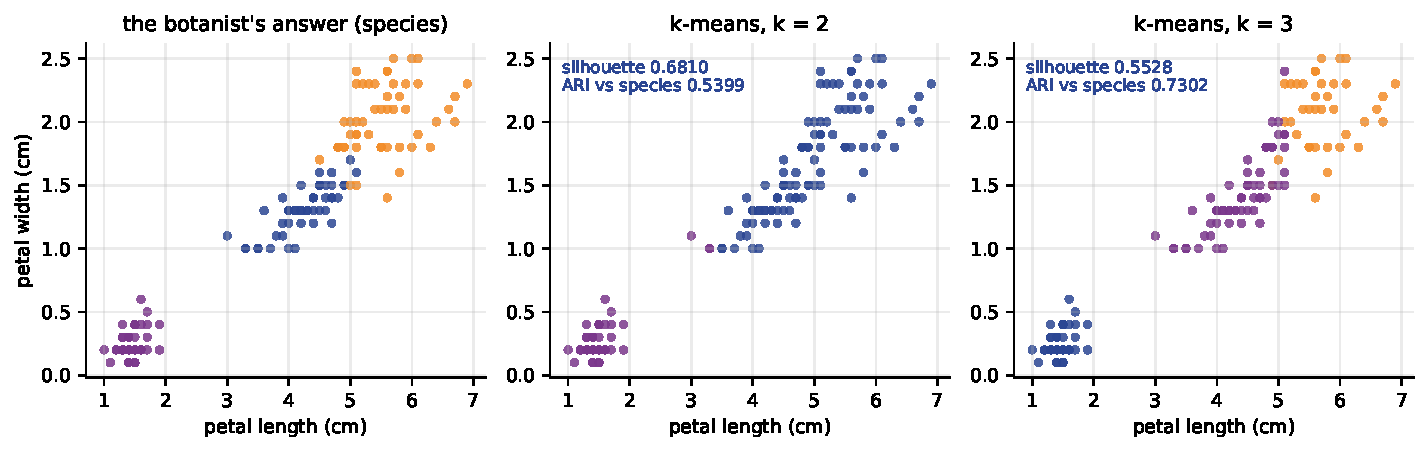
\includegraphics[width=\textwidth]{twoanswers.pdf}
  \caption{One dataset, three groupings. Left: the species, which a botanist
  supplies from outside the data. Middle and right: what k-means returns for
  $k=2$ and $k=3$. \emph{Setosa} is genuinely far from the other two, and the
  other two genuinely touch --- so a score that rewards separation merges
  them and a score that knows the species does not.}
  \label{fig:twoanswers}
\end{figure}

\begin{keyidea}
The silhouette is not wrong about iris. It is answering its own question ---
\emph{are these clusters well separated?} --- correctly, and the honest answer
is that \emph{versicolor} and \emph{virginica} are not well separated in these
four measurements. It is simply not answering the botanist's question. When an
internal index and a set of labels disagree, the useful move is to ask what
each of them is measuring, not to declare one of them broken.
\end{keyidea}

\subsection{The same lesson again: scaling is the definition of ``similar''}
\label{sec:scaling}

The iris example is subtle because both answers are close. Here is a blunter
one. \texttt{load\_wine} has $178$ bottles, $13$ chemical measurements, and
three known cultivars. Run k-means with $k = 3$ twice: once on the raw table,
once after standardising every column.

\begin{lstlisting}
from sklearn.preprocessing import StandardScaler
raw = KMeans(n_clusters=3, n_init=10, random_state=0).fit_predict(Xw)
std = KMeans(n_clusters=3, n_init=10, random_state=0).fit_predict(
          StandardScaler().fit_transform(Xw))
\end{lstlisting}
\begin{codeout}
column ranges in the raw table
   alcohol                  min    11.03  max    14.83  sd     0.81
   magnesium                min    70.00  max   162.00  sd    14.24
   color_intensity          min     1.28  max    13.00  sd     2.31
   proline                  min   278.00  max  1680.00  sd   314.02
unscaled: silhouette in its own space 0.5711, ARI vs cultivar 0.3711
scaled  : silhouette in its own space 0.2849, ARI vs cultivar 0.8975
agreement between the two clusterings: ARI 0.3543
\end{codeout}

Standardising takes the agreement with the true cultivar from
$\mathbf{0.3711}$ to $\mathbf{0.8975}$, and the two clusterings agree with
each other at only $0.3543$ --- barely better than half. One preprocessing
decision, made in one line, produced two substantially different pictures of
the same $178$ bottles.

The reason is arithmetic:

\begin{codeout}
share of the raw total variance held by each column
   proline                    98609.60  (99.77%)
   magnesium                    202.84  ( 0.21%)
   alcalinity_of_ash             11.09  ( 0.01%)
   color_intensity                5.34  ( 0.01%)
   top column alone accounts for 99.77% of the distance budget
\end{codeout}

\texttt{proline} runs into the thousands while \texttt{alcohol} runs from $11$
to $15$. Squared Euclidean distance on the raw table is
$\mathbf{99.77\%}$ a comparison of proline; the other twelve columns are
decoration.

\begin{caution}[The silhouettes above are not comparable]
$0.5711$ and $0.2849$ were computed in \emph{different spaces}. An internal
index measures how good a partition is \emph{given a distance}; change the
distance and you have changed the ruler as well as the thing being measured.
Never compare an internal index across two different feature scalings, two
different distance metrics, or two different feature subsets --- and be
suspicious of anybody who does.
\end{caution}

\begin{figure}[htbp]
  \centering
  
\includegraphics[width=\textwidth]{scaling.pdf}
  \caption{The same $178$ bottles, projected onto the first two principal
  components of the standardised table so that all three panels are drawn in
  one space. Left, the cultivars. Middle, k-means on the raw table, which is
  substantially a one-dimensional split on proline. Right, k-means after
  standardising.}
  \label{fig:scaling}
\end{figure}

\subsection{What ``exploratory'' means}

Put the two demonstrations together. Clustering does not \emph{discover} a
grouping that was already there; it \emph{proposes} one, and the proposal is a
joint consequence of the data, the distance, the algorithm and the settings.
Vladimir Estivill-Castro put it in one line in 2002:
\emph{clustering is in the eye of the beholder}.

That is not a licence to be sloppy --- it is the opposite. Because there is no
answer key, the burden of stating your assumptions falls entirely on you. A
defensible clustering result is one that comes with:

\begin{enumerate}[leftmargin=*]
  \item the distance used, and the scaling that produced it;
  \item the algorithm and the settings, including how $k$ was chosen;
  \item at least two internal indices, \emph{including the ones that
    disagreed};
  \item a look at the actual clusters --- their sizes, their centroids, a few
    members of each;
  \item a statement of what the groups will be used for.
\end{enumerate}

\begin{tryit}
Run the wine comparison yourself and add a third variant: scale with
\texttt{MinMaxScaler} instead of \texttt{StandardScaler}. You should find a
third clustering, different again from both. Then ask the question these notes
keep asking: which one is right? There is no answer, and noticing that there
is no answer is the point of this section.
\end{tryit}

\notesources{\AMLUnitVIISources}

% =========================================================================
\section{The taxonomy of clustering algorithms}
\label{sec:tax}

\subsection{Five families}

The literature contains hundreds of clustering algorithms. They fall into five
families, and the families differ in what they \emph{assume a cluster looks
like}. That assumption is the thing to remember; the implementation details
come in the later lectures.

\begin{center}
\small
\begin{tabular}{@{}lp{5.0cm}p{5.0cm}@{}}
  \toprule
  \textbf{Family} & \textbf{Mechanism} & \textbf{Assumed shape} \\
  \midrule
  \textbf{Partitioning} &
    choose $k$ representatives, assign each point to the nearest, move the
    representatives, repeat until stable. \emph{k-means, k-medoids, CLARA.} &
    convex, roughly spherical, roughly equal size; one centre each. The
    boundary between two clusters is always a hyperplane. \\[0.3em]
  \textbf{Hierarchical} &
    repeatedly merge the two closest clusters (agglomerative) or repeatedly
    split (divisive), producing a dendrogram. \emph{HAC with single,
    complete, average or Ward linkage.} &
    whatever the linkage assumes. Ward behaves like k-means; single linkage
    assumes clusters are \emph{connected chains} and will happily produce a
    long thin one. \\[0.3em]
  \textbf{Density-based} &
    a cluster is a maximal set of points connected through regions whose local
    density exceeds a threshold. \emph{DBSCAN, OPTICS, DENCLUE.} &
    dense regions separated by sparse ones. \textbf{Shape is unconstrained.}
    Density is assumed roughly uniform within a run. Points in sparse regions
    are left out as noise. \\[0.3em]
  \textbf{Grid-based} &
    quantise the space into cells, summarise each cell, then cluster the
    cells. \emph{STING, CLIQUE, WaveCluster.} &
    as density-based, plus the assumption that a \emph{fixed resolution} is
    adequate. Fast: cost is driven by the number of cells, not the number of
    points. \\[0.3em]
  \textbf{Model-based} &
    assume the data was generated by a mixture of distributions and fit the
    mixture by maximum likelihood, usually with EM. \emph{Gaussian mixture
    models, latent class models.} &
    whatever family you assumed. A full-covariance Gaussian mixture assumes
    \textbf{ellipsoidal} clusters of arbitrary orientation and size, which is
    strictly more general than k-means. \\
  \bottomrule
\end{tabular}
\end{center}

\subsection{Measured: four shapes, five algorithms}
\label{sec:shapes}

A taxonomy is only worth learning if the distinctions do something. Here are
four two-dimensional problems, each with a known generating group structure,
and five algorithms run on each. The score is the adjusted Rand index against
the generating groups --- $1.0000$ is perfect, $0.0000$ is chance.

\begin{lstlisting}
Xb, yb = make_blobs(n_samples=500, centers=3, cluster_std=1.0,
                    random_state=170)                       # spherical
Xa, ya = make_blobs(n_samples=500, random_state=170)
Xa = Xa @ np.array([[0.60, -0.60], [-0.40, 0.80]])          # elongated
Xv, yv = make_blobs(n_samples=500, cluster_std=[1.0, 2.5, 0.5],
                    random_state=170)                       # unequal spread
Xm, ym = make_moons(n_samples=500, noise=0.06, random_state=7)
\end{lstlisting}
\begin{codeout}
dataset (ARI)        KMeans      Ward    Single  GaussMix    DBSCAN
spherical blobs      1.0000    1.0000    0.5682    1.0000    0.9910
elongated blobs      0.5554    0.5281    0.5682    1.0000    0.9970
unequal spread       0.7872    0.8692    0.0002    0.9468    0.8054
two moons            0.2445    0.3447    1.0000    0.5003    1.0000
no column wins every row
\end{codeout}

\begin{figure}[htbp]
  \centering
  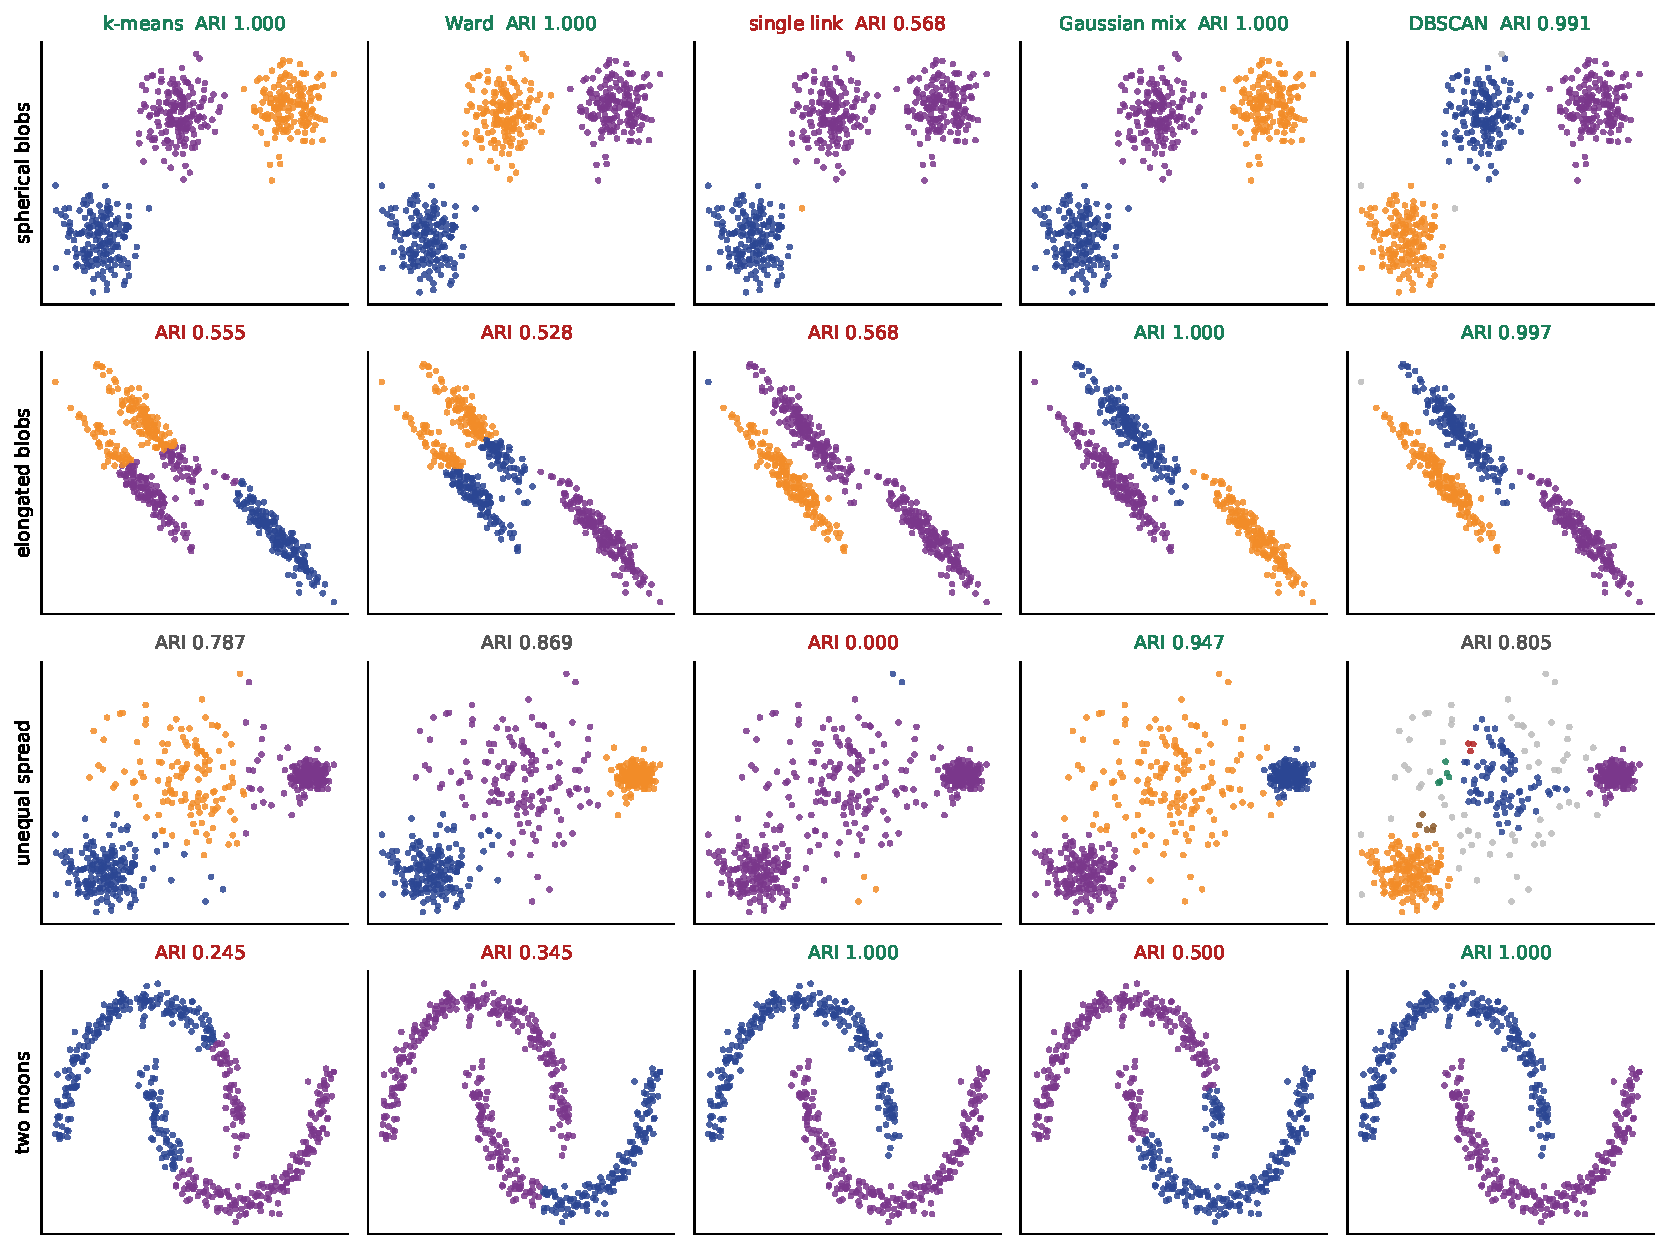
\includegraphics[width=0.86\textwidth]{shapes.pdf}
  \caption{The taxonomy with teeth. Rows are the four problems, columns the
  five algorithms; each panel is titled with its adjusted Rand index, green
  above $0.9$ and red below $0.6$. Every column contains at least one red
  panel.}
  \label{fig:shapes}
\end{figure}

Four things to take from that table.

\textbf{k-means fails on the moons, and fails confidently.} It scores
$0.2445$. The reason is structural rather than a matter of tuning: k-means
assigns each point to the nearest centre, so the boundary between two clusters
is the perpendicular bisector of their centres --- a straight line. Two
interleaved crescents cannot be separated by a straight line. What makes this
dangerous is that k-means does not complain. It returns two clean-looking
clusters and no warning.

\textbf{DBSCAN succeeds on the moons, exactly.} ARI $1.0000$. It never asks
where the centre of a cluster is; it grows a cluster through any connected
dense region, and a crescent is a connected dense region.

\textbf{The Gaussian mixture succeeds on the elongated blobs where k-means
fails.} $1.0000$ against $0.5554$. Rotating and stretching the blobs breaks
k-means' spherical assumption but not the mixture's ellipsoidal one. This is
the clearest illustration of what ``model-based'' buys: a strictly larger
family of admissible cluster shapes.

\textbf{Single linkage is a knife with no handle.} Perfect on the moons
($1.0000$), catastrophic when the clusters have unequal spread
($\mathbf{0.0002}$, which is chance). It merges whichever two clusters have
the single closest pair of points, so one stray point in the gap
\emph{chains} two clusters into one. On the wide cluster of the third dataset
that happens immediately.

And DBSCAN's own weakness is in the same row: $0.8054$ on unequal spread, its
worst result, with $68$ of $500$ points discarded as noise.

\begin{codeout}
spherical blobs   eps=1.00 -> 3 clusters,   3 points called noise
elongated blobs   eps=0.50 -> 3 clusters,   1 points called noise
unequal spread    eps=0.75 -> 6 clusters,  68 points called noise
two moons         eps=0.20 -> 2 clusters,   0 points called noise
\end{codeout}

A single density threshold cannot fit clusters of genuinely different density:
set it loose enough for the sparse cluster and the dense ones merge; set it
tight enough for the dense ones and the sparse one dissolves into noise. Here
it found six clusters where there are three.

\begin{keyidea}
There is no default clustering algorithm. Choosing one is choosing a shape
assumption, and the assumption is a claim about your data that you should be
able to defend. If you cannot say what shape you expect your clusters to be,
plot the data before you cluster it.
\end{keyidea}

\subsection{A grid clusterer, built from scratch}
\label{sec:grid}

Grid methods sound exotic and are not. Here is a complete one, in three steps:
lay a $G \times G$ grid over the data, keep the cells containing at least
$\tau$ points, and treat each connected group of surviving cells as a cluster.

\begin{lstlisting}
def grid_cluster(X, G=10, tau=3):
    lo, hi = X.min(axis=0) - 1e-9, X.max(axis=0) + 1e-9
    idx = np.clip(((X - lo) / (hi - lo) * G).astype(int), 0, G - 1)
    counts = np.zeros((G, G), dtype=int)
    for a, b in idx: counts[a, b] += 1
    dense = counts >= tau
    comp, ncomp = ndimage.label(dense, structure=np.ones((3, 3)))
    labels = np.array([comp[a, b] - 1 if dense[a, b] else -1 for a, b in idx])
    return labels, counts, dense, ncomp
\end{lstlisting}
\begin{codeout}
cell counts, x across, y up (a dot = fewer than tau = 3)
      .   .  13  21  10   .   .   .   .   .
      .  17   8   6  20  12   .   .   .   .
      4  11   .   .   .  17   3   .   .   .
     17   3   .   7   .   5  11   .   .   6
     14   .   .  12   .   .  11   .   .  15
     12   .   .  16   .   .  16   .   .  11
      9   .   .  10   6   .   6   .   .  19
      .   .   .   4  16   .   .   .  16   4
      .   .   .   .  14  19   6  17  14   .
      .   .   .   .   .   5  19   9   .   .
connected dense regions: 2
\end{codeout}

You can see the two crescents in the printed table with your eyes. Forty-three
of the hundred cells survive the threshold and they fall into exactly two
connected regions, giving ARI $\mathbf{0.9643}$ with nine points discarded as
noise. The whole algorithm is a two-dimensional histogram plus a flood fill,
and it never computes a single pairwise distance.

That is the advantage of the family: the cost depends on the number of
\emph{cells}, not the number of points, so a grid method scales to data that a
distance-matrix method cannot touch. The disadvantage is on the next line.

\begin{codeout}
G=10 tau=3  dense cells  43/100  clusters 2  noise  9  ARI 0.9643
G=12 tau=2  dense cells  56/144  clusters 1  noise  9  ARI 0.0000
G=14 tau=2  dense cells  73/196  clusters 2  noise 13  ARI 0.9486
G=14 tau=3  dense cells  62/196  clusters 2  noise 35  ARI 0.8646
\end{codeout}

\begin{caution}[A grid clusterer is brittle at its resolution]
Loosen the threshold by one point, from $\tau = 3$ to $\tau = 2$ at
$G = 12$, and a single cell between the two arms becomes dense. The two
regions connect, the answer becomes ``one cluster'', and the ARI collapses
from $0.9643$ to $\mathbf{0.0000}$. Nothing warned; the algorithm ran
successfully and returned a wrong answer. Whenever you use a method with a
resolution parameter, run it at several resolutions and look at the whole
range before believing any single one.
\end{caution}

\begin{figure}[htbp]
  \centering
  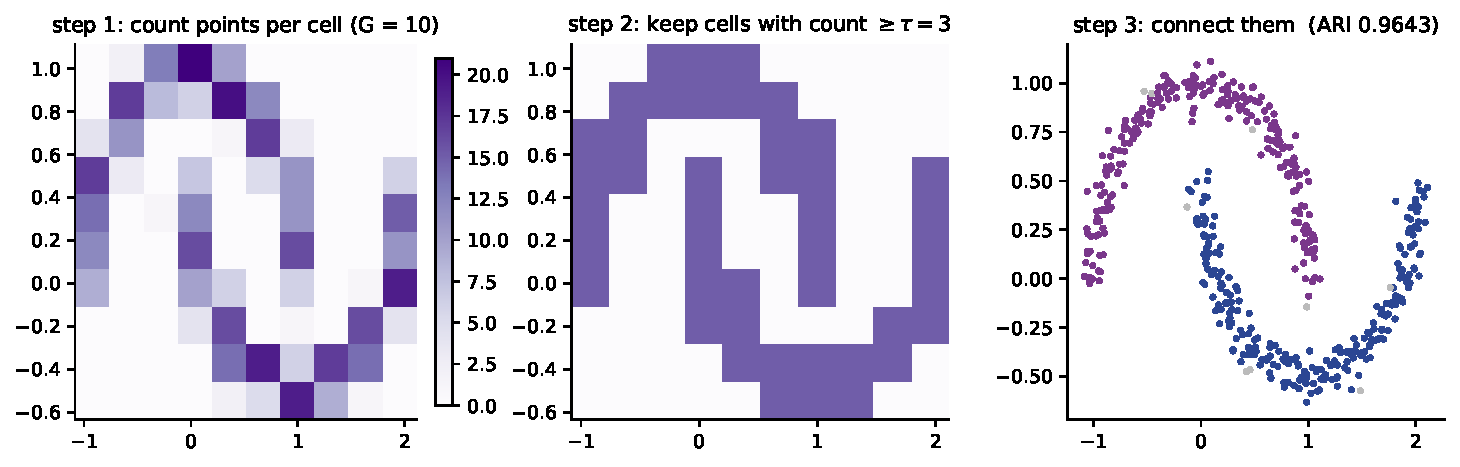
\includegraphics[width=\textwidth]{gridclust.pdf}
  \caption{A grid clusterer in three steps: count, threshold, connect.}
  \label{fig:grid}
\end{figure}

\notesources{\AMLUnitVIISources}

% =========================================================================
\section{The statistics of cluster analysis}
\label{sec:stats}

Whatever algorithm produced a clustering, the same handful of quantities
describe it. They are the vocabulary of the rest of the unit and the source of
most examination arithmetic.

\subsection{The cluster centroid}

The \textbf{centroid} of cluster $C_j$ is the componentwise mean of its
members,
\begin{equation}
  c_j = \frac{1}{n_j} \sum_{x \in C_j} x .
  \label{eq:centroid}
\end{equation}
It is a point in $\mathbb{R}^d$ and it need not be one of the data points ---
the centroid of two flowers is generally not a flower. (When you insist that
the representative \emph{be} a data point you get the \textbf{medoid} instead,
and the algorithm becomes k-medoids, which a later lecture in this unit
covers.)

The centroid has a property that everything below depends on: it is the point
that minimises the sum of squared distances to the members of the cluster.
For any $m \in \mathbb{R}^d$,
\begin{equation}
  \sum_{x \in C_j} \lVert x - m \rVert^2
    = \sum_{x \in C_j} \lVert x - c_j \rVert^2 + n_j \lVert c_j - m \rVert^2 .
  \label{eq:shift}
\end{equation}
The second term is non-negative and vanishes only at $m = c_j$. We prove this
in Section~\ref{sec:proof}; it is a two-line expansion and it does all the
work.

\begin{lstlisting}
km3 = KMeans(n_clusters=3, n_init=10, random_state=0).fit(X)
print(km3.cluster_centers_, X.mean(axis=0))
\end{lstlisting}
\begin{codeout}
cluster centroids on the four iris measurements
        sepal len    sepal wid    petal len    petal wid      n
  c0       5.901613     2.748387     4.393548     1.433871   62
  c1       5.006000     3.428000     1.462000     0.246000   50
  c2       6.850000     3.073684     5.742105     2.071053   38
grand     5.843333     3.057333     3.758000     1.199333
\end{codeout}

A centroid is also the most useful \emph{description} of a cluster you have.
Cluster \texttt{c1} has petals of length $1.46$\,cm; the other two have petals
of $4.39$ and $5.74$\,cm. That single column says immediately what the
clustering found. When you report a clustering, report the centroids.

\subsection{Within, between, and total}

Three sums of squares. Let $\bar{x}$ be the grand mean of all $n$ points.

\begin{align}
  T &= \sum_{i=1}^{n} \lVert x_i - \bar{x} \rVert^2
      && \text{\textbf{total scatter}: a property of the data alone}
      \label{eq:T}\\[0.2em]
  W &= \sum_{j=1}^{k} \sum_{x \in C_j} \lVert x - c_j \rVert^2
      && \text{\textbf{within-cluster sum of squares} (WCSS): tightness}
      \label{eq:W}\\[0.2em]
  B &= \sum_{j=1}^{k} n_j \lVert c_j - \bar{x} \rVert^2
      && \text{\textbf{between-cluster sum of squares} (BCSS): separation}
      \label{eq:B}
\end{align}

Note carefully what each does and does not depend on. $T$ contains no
reference to the clustering at all --- change $C$ and $T$ does not move.
$W$ is small when the clusters are tight. $B$ is large when the centroids are
spread out, and it weights each centroid by the size of its cluster, so
moving a large cluster away from the grand mean contributes more than moving a
small one.

\subsection{The decomposition, and why it matters}
\label{sec:decomp}

\begin{keyidea}[The identity everything rests on]
\[
  T = W + B .
\]
The total scatter of a dataset splits exactly into a within-cluster part and a
between-cluster part, for \emph{any} clustering. Since $T$ is fixed by the
data, \textbf{minimising $W$ and maximising $B$ are the same problem}. That is
why k-means only ever mentions $W$, and why every index in
Section~\ref{sec:valid} is built out of these two numbers.
\end{keyidea}

\subsubsection*{The proof}
\label{sec:proof}

Take a single cluster $C_j$ and put $m = \bar{x}$ in equation~\eqref{eq:shift}.
Expanding the left side directly:
\[
  \sum_{x \in C_j} \lVert x - \bar{x} \rVert^2
  = \sum_{x \in C_j} \lVert (x - c_j) + (c_j - \bar{x}) \rVert^2
  = \sum_{x \in C_j} \lVert x - c_j \rVert^2
  + 2 (c_j - \bar{x})^{\!\top}\!\!\sum_{x \in C_j}(x - c_j)
  + n_j \lVert c_j - \bar{x} \rVert^2 .
\]
The middle term vanishes, because $\sum_{x \in C_j}(x - c_j) = 0$ by the
definition of the centroid in equation~\eqref{eq:centroid} --- that is the
\emph{only} property of the centroid used anywhere in this argument. So
\[
  \sum_{x \in C_j} \lVert x - \bar{x} \rVert^2
  = \sum_{x \in C_j} \lVert x - c_j \rVert^2 + n_j \lVert c_j - \bar{x}\rVert^2 .
\]
Now sum over $j = 1, \dots, k$. The clusters partition the data, so the left
side sums to $T$; the right side sums to $W + B$. \ensuremath{\square}

The proof also tells you when the identity fails: it needs $c_j$ to be exactly
the mean of $C_j$. Compute $W$ around medoids, or around centroids from a
previous iteration, and $T = W + B$ stops holding. If your numbers do not add
up, that is the first thing to check.

\subsection{Six points, by hand}
\label{sec:byhand}

\begin{worked}[The whole decomposition on six points]
Take six points in the plane:
\[
  P_1(2,2)\quad P_2(4,2)\quad P_3(3,5)\quad
  P_4(9,3)\quad P_5(11,3)\quad P_6(10,6).
\]
The grand mean is
$\bar{x} = \bigl(\tfrac{2+4+3+9+11+10}{6}, \tfrac{2+2+5+3+3+6}{6}\bigr)
 = (6.5,\ 3.5)$.

\medskip
\textbf{Clustering A --- left three against right three.}
\[
  c_1 = \Bigl(\tfrac{2+4+3}{3},\ \tfrac{2+2+5}{3}\Bigr) = (3,\,3),
  \qquad
  c_2 = \Bigl(\tfrac{9+11+10}{3},\ \tfrac{3+3+6}{3}\Bigr) = (10,\,4).
\]
Within, cluster by cluster. Offsets from $(3,3)$ are $(-1,-1)$, $(1,-1)$,
$(0,2)$, contributing $2 + 2 + 4 = 8$. Offsets from $(10,4)$ are the same
three vectors, contributing another $8$. So
\[
  W_A = 8 + 8 = \mathbf{16}.
\]
Between. Both centroids sit at squared distance
$3.5^2 + 0.5^2 = 12.25 + 0.25 = 12.5$ from the grand mean, and each has three
members:
\[
  B_A = 3(12.5) + 3(12.5) = \mathbf{75}.
\]
Total, computed independently from the grand mean:
\[
  T = 22.5 + 8.5 + 14.5 + 6.5 + 20.5 + 18.5 = \mathbf{91},
\]
taking the six terms in order $P_1$ to $P_6$. And $16 + 75 = 91$. \checkmark

\medskip
\textbf{Clustering B --- low $y$ against high $y$.} Put
$\{P_1,P_2,P_4,P_5\}$ in one cluster and $\{P_3,P_6\}$ in the other:
\[
  c_1 = (6.5,\,2.5), \qquad c_2 = (6.5,\,5.5).
\]
Within: $20.5 + 6.5 + 6.5 + 20.5 = 54$ for the first, $12.5 + 12.5 = 25$ for
the second, so $W_B = \mathbf{79}$. Between:
$4 \times 1 + 2 \times 4 = \mathbf{12}$. And $79 + 12 = 91$ again.
\end{worked}

That pair of calculations is the whole section. \textbf{The same $T$; two
completely different splits of it.} Clustering A is tight and well separated
($16 \mid 75$); clustering B is loose and overlapping ($79 \mid 12$). The
decomposition is the instrument that says so, and it is the reason we can rank
two clusterings at all without an answer key.

\begin{lstlisting}
def scatter_decomposition(X, labels):
    g = X.mean(axis=0)
    total = ((X - g) ** 2).sum()
    within = between = 0.0
    for c in np.unique(labels):
        M = X[labels == c]; ck = M.mean(axis=0)
        within  += ((M - ck) ** 2).sum()
        between += len(M) * ((ck - g) ** 2).sum()
    return total, within, between
\end{lstlisting}
\begin{codeout}
clustering              T        W        B        W+B
A: left/right       91.00    16.00    75.00      91.00
B: low/high y       91.00    79.00    12.00      91.00
T does not depend on the clustering; W and B trade off inside it
\end{codeout}

\begin{figure}[htbp]
  \centering
  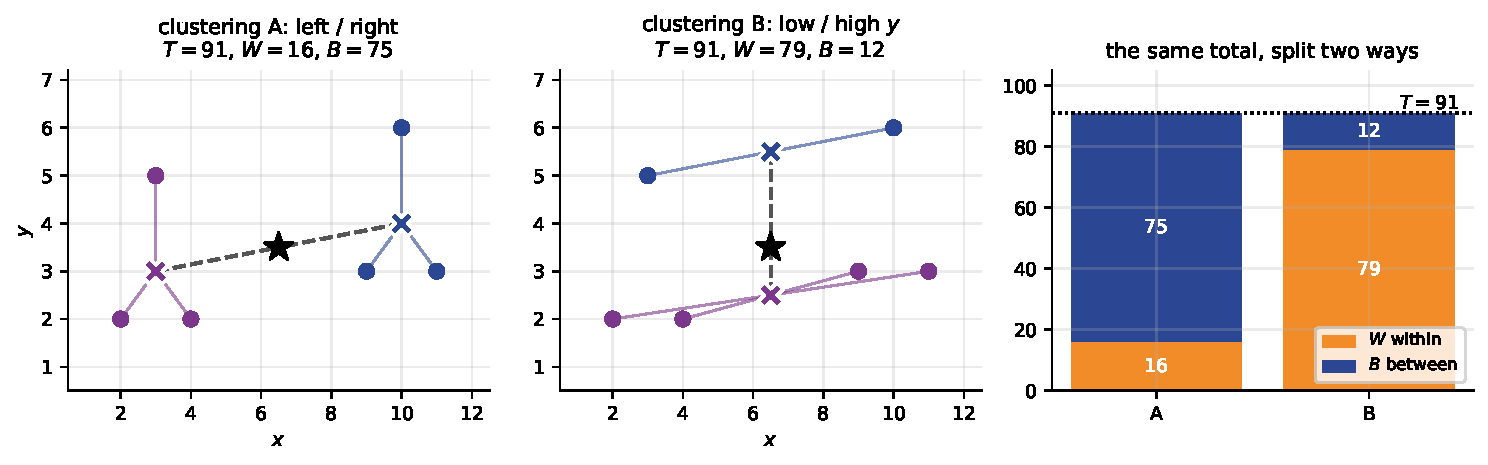
\includegraphics[width=\textwidth]{decomp.pdf}
  \caption{The six points under both clusterings. Coloured lines are the
  within-cluster displacements that make $W$; dashed grey lines run from each
  centroid to the grand mean (the black star) and make $B$. Right: a fixed
  budget of $T = 91$, divided two ways.}
  \label{fig:decomp}
\end{figure}

One more check worth doing once. k-means with $k = 2$ on these six points
recovers clustering A, and its \texttt{inertia\_} attribute is exactly the $W$
you computed:

\begin{codeout}
k-means centroids (sorted by x)
   (3.00, 3.00)
   (10.00, 4.00)
k-means labels         [1 1 1 0 0 0]
our clustering A       [0 0 0 1 1 1]
k-means inertia_      16.0000
our W for clustering A 16.0000
\end{codeout}

Note that the labels are $[1\,1\,1\,0\,0\,0]$ where ours were
$[0\,0\,0\,1\,1\,1]$. Same partition, different names. Cluster identifiers
carry no meaning; Section~\ref{sec:external} makes that precise.

\subsection{Verified on real data, at every $k$}

\begin{lstlisting}
for k in range(1, 9):
    km = KMeans(n_clusters=k, n_init=10, random_state=0).fit(X)
    T, W, B = scatter_decomposition(X, km.labels_)
    print(k, T, W, B, abs(T - W - B))
\end{lstlisting}
\begin{codeout}
  k              T              W              B      |T-W-B|
  1     681.370600     681.370600       0.000000    0.000e+00
  2     681.370600     152.347952     529.022648    1.137e-13
  3     681.370600      78.851441     602.519159    0.000e+00
  4     681.370600      57.228473     624.142127    1.137e-13
  5     681.370600      46.446182     634.924418    0.000e+00
  6     681.370600      39.039987     642.330613    1.137e-13
  7     681.370600      34.420192     646.950408    0.000e+00
  8     681.370600      30.064593     651.306007    0.000e+00
\end{codeout}

$T = 681.370600$ in every row, and the largest residual is
$1.137 \times 10^{-13}$ --- double-precision rounding, not mathematics. At
$k = 1$ everything is within and nothing is between. As $k$ grows the budget
migrates from $W$ into $B$.

\subsection{Why $W$ cannot choose $k$}
\label{sec:elbow}

\begin{caution}[``Pick the $k$ with the smallest $W$'' returns $k = n$]
$W$ is monotone decreasing in $k$. Splitting any cluster into two can only
decrease $W$ (by equation~\eqref{eq:shift}, the two new centroids each fit
their own members at least as well as the old one did), and at $k = n$ every
point is its own centroid so $W = 0$ exactly. \textbf{Minimising $W$ is not an
objective, it is a countdown.} The same argument, mirrored, says $B/T$ climbs
monotonically to $1$.
\end{caution}

\begin{codeout}
  k            W     inertia_        B/T           CH
  2   152.347952   152.347952     0.7764     513.9245
  3    78.851441    78.851441     0.8843     561.6278
  4    57.228473    57.228473     0.9160     530.7658
  5    46.446182    46.446182     0.9318     495.5415
  6    39.039987    39.039987     0.9427     473.8506
  7    34.420192    34.420192     0.9495     447.9634
  8    30.064593    30.064593     0.9559     439.4607
W falls at every step; it can never choose k on its own
\end{codeout}

The middle column is scikit-learn's \texttt{inertia\_}, which agrees with our
$W$ to every printed digit --- \texttt{inertia\_} \emph{is} the
within-cluster sum of squares, nothing more.

The traditional response is the \textbf{elbow method}: plot $W$ against $k$
and look for the point where the curve stops falling steeply. On iris that
suggests $k = 3$, and here that happens to be a good answer. But be honest
about what it is. It is a visual judgement on a curve that has no
mathematical optimum, two people reading the same plot routinely name
different elbows, and on many real datasets the curve is a smooth arc with no
elbow at all. Use it to generate candidates, and then justify the choice with
something else.

\begin{figure}[htbp]
  \centering
  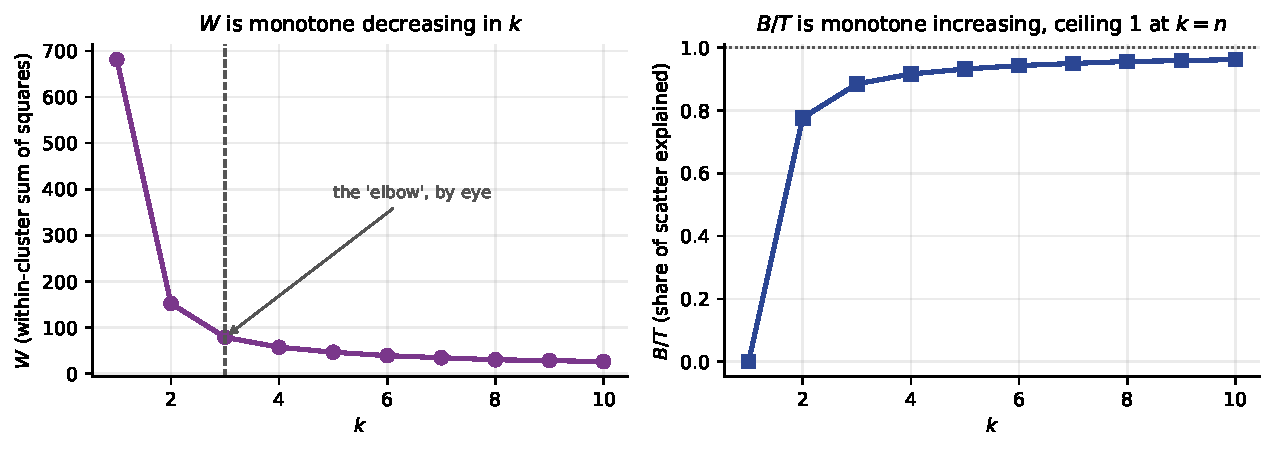
\includegraphics[width=\textwidth]{elbow.pdf}
  \caption{$W$ falls monotonically towards zero and $B/T$ climbs
  monotonically towards one. Neither curve has an interior optimum, so
  neither can select $k$ by itself.}
  \label{fig:elbow}
\end{figure}

\subsection{Calinski--Harabasz: the decomposition with the penalty put back}
\label{sec:ch}

The fix is to charge for the clusters you use. The
\textbf{Calinski--Harabasz index}, sometimes called the variance ratio
criterion, divides each sum of squares by its degrees of freedom:
\begin{equation}
  \mathrm{CH} = \frac{B / (k-1)}{W / (n-k)} .
  \label{eq:ch}
\end{equation}
Higher is better. Adding a cluster increases $B$, but it also spends a degree
of freedom, and past the useful point the numerator stops growing fast enough
to pay for it. Unlike $W$, this index has an interior maximum.

\begin{worked}[CH on the six points]
Clustering A: $B = 75$, $W = 16$, $k = 2$, $n = 6$, so
\[
  \mathrm{CH}_A = \frac{75/(2-1)}{16/(6-2)} = \frac{75}{4} = \mathbf{18.75}.
\]
Clustering B: $B = 12$, $W = 79$, so
$\mathrm{CH}_B = \dfrac{12}{79/4} = \dfrac{48}{79} = \mathbf{0.6076}$.
Clustering A is about thirty times better by this measure.
\end{worked}

\begin{codeout}
A: left/right     B/T = 0.8242   CH by hand =  18.7500   sklearn =  18.7500
B: low/high y     B/T = 0.1319   CH by hand =   0.6076   sklearn =   0.6076
k=3  B/(k-1) = 301.259579   W/(n-k) =   0.536404   ratio =  561.6278
     sklearn calinski_harabasz_score = 561.6278
k=6  B/(k-1) = 128.466123   W/(n-k) =   0.271111   ratio =  473.8506
     sklearn calinski_harabasz_score = 473.8506
\end{codeout}

\begin{tryit}
Compute $\mathrm{CH}$ by hand for the iris clustering at $k = 2$: you have
$B = 529.022648$, $W = 152.347952$, $n = 150$. You should get
$\frac{529.022648}{152.347952/148} = 513.92$, matching the table in
Section~\ref{sec:twoiris}. If you get something near $3.47$ you forgot the
degrees of freedom.
\end{tryit}

\notesources{\AMLUnitVIISources}

% =========================================================================
\section{Internal and external validation}
\label{sec:valid}

\subsection{Two kinds of validation, and only one is usually available}

\textbf{Internal} validation scores a clustering using nothing but the points
and the assignments. No labels anywhere. This is what you actually have on a
real problem, and it is what Sections~\ref{sec:silhand} to \ref{sec:allthree}
develop: the silhouette, Calinski--Harabasz, Davies--Bouldin.

\textbf{External} validation compares your clustering to a known grouping
supplied from outside. It requires a label column you did not use for
fitting, which on real clustering problems you do not have. We use it here
because \texttt{load\_iris} happens to ship with one --- which lets us do
something valuable: \emph{check the internal measures against a known answer
and find out where they are wrong}.

\begin{caution}[Do not use external validation as your objective]
If you have labels for all your rows, you have a classification problem, not a
clustering problem, and you should be training a classifier. External indices
in these notes are a diagnostic instrument for studying internal indices, not
a model-selection criterion you can use in the field.
\end{caution}

\subsection{The silhouette, by hand}
\label{sec:silhand}

For each point $i$ in cluster $C_j$ define
\begin{equation}
  a(i) = \frac{1}{n_j - 1}\!\!\sum_{x \in C_j,\, x \neq i}\!\! d(i, x),
  \qquad
  b(i) = \min_{l \neq j}\ \frac{1}{n_l}\sum_{x \in C_l} d(i, x),
  \qquad
  s(i) = \frac{b(i) - a(i)}{\max\{a(i),\, b(i)\}} .
  \label{eq:sil}
\end{equation}
In words: $a(i)$ is the average distance to the point's own cluster-mates,
$b(i)$ the average distance to the members of the \emph{nearest other}
cluster. If $a$ is much smaller than $b$ then $s$ is near $+1$ and the point
is comfortably placed. If they are equal $s$ is $0$ and the point is on the
border. \textbf{If $a > b$ then $s$ is negative and the point is on average
closer to another cluster's members than to its own} --- the clearest single
signal that it has been misassigned. Singleton clusters are defined to have
$s = 0$.

The \textbf{silhouette score} of a clustering is the mean of $s(i)$ over all
points.

\begin{worked}[$s(P_1)$ under clustering A]
The pairwise distances among the six points of Section~\ref{sec:byhand}:
\begin{codeout}
            P1      P2      P3      P4      P5      P6
  P1    0.0000  2.0000  3.1623  7.0711  9.0554  8.9443
  P2    2.0000  0.0000  3.1623  5.0990  7.0711  7.2111
  P3    3.1623  3.1623  0.0000  6.3246  8.2462  7.0711
  P4    7.0711  5.0990  6.3246  0.0000  2.0000  3.1623
  P5    9.0554  7.0711  8.2462  2.0000  0.0000  3.1623
  P6    8.9443  7.2111  7.0711  3.1623  3.1623  0.0000
\end{codeout}
$P_1$ is in the cluster $\{P_1,P_2,P_3\}$, so
\[
  a(P_1) = \frac{d(P_1,P_2) + d(P_1,P_3)}{2}
         = \frac{2 + 3.162278}{2} = \frac{5.162278}{2} = 2.581139 .
\]
The only other cluster is $\{P_4,P_5,P_6\}$, so
\[
  b(P_1) = \frac{7.071068 + 9.055385 + 8.944272}{3}
         = \frac{25.070725}{3} = 8.356908 .
\]
Since $b > a$, the denominator is $b$, and
\[
  s(P_1) = \frac{8.356908 - 2.581139}{8.356908}
         = \frac{5.775769}{8.356908} = \mathbf{0.691137}.
\]
\end{worked}

\begin{lstlisting}
from scipy.spatial.distance import cdist
from sklearn.metrics import silhouette_samples, silhouette_score
D = cdist(P6, P6)
s = silhouette_samples(P6, LAB_A)
for i in range(6):
    same = D[i][LAB_A == LAB_A[i]]
    a = same.sum() / (len(same) - 1)
    b = D[i][LAB_A != LAB_A[i]].mean()
    print(i + 1, a, b, (b - a) / max(a, b), s[i])
\end{lstlisting}
\begin{codeout}
point       a(i)      b(i)      s(i)   sklearn
  P1    2.581139  8.356908  0.691137  0.691137
  P2    2.581139  6.460397  0.600467  0.600467
  P3    3.162278  7.213945  0.561644  0.561644
  P4    2.581139  6.164881  0.581316  0.581316
  P5    2.581139  8.124221  0.682291  0.682291
  P6    3.162278  7.742147  0.591550  0.591550
mean silhouette  0.618068   sklearn 0.618068
clustering B     -0.071164   sklearn -0.071164
\end{codeout}

Two things. Our hand arithmetic and \texttt{silhouette\_samples} agree in
every digit shown; the library is doing exactly equation~\eqref{eq:sil} and
nothing else. And clustering B scores $\mathbf{-0.071164}$ --- negative,
meaning the average point of that partition is nearer the other cluster's
members than its own. The silhouette does not merely prefer A to B; it says B
is actively wrong.

\subsection{Silhouette on real data, and the profile}

\begin{codeout}
k=2  mean 0.6810   negative silhouettes: 0 of 150   min 0.0407
     cluster 0  n= 53  mean s = 0.7695
     cluster 1  n= 97  mean s = 0.6327
k=3  mean 0.5528   negative silhouettes: 0 of 150   min 0.0264
     cluster 0  n= 62  mean s = 0.4173
     cluster 1  n= 50  mean s = 0.7981
     cluster 2  n= 38  mean s = 0.4511
\end{codeout}

The per-cluster breakdown is more informative than the mean. At $k = 3$ the
three clusters score $0.4173$, $\mathbf{0.7981}$ and $0.4511$: one crisp
cluster --- \emph{setosa}, cluster $1$, with $50$ members --- and two mediocre
ones that are really one region cut in half. A mean of $0.5528$ conceals that
completely.

\begin{figure}[htbp]
  \centering
  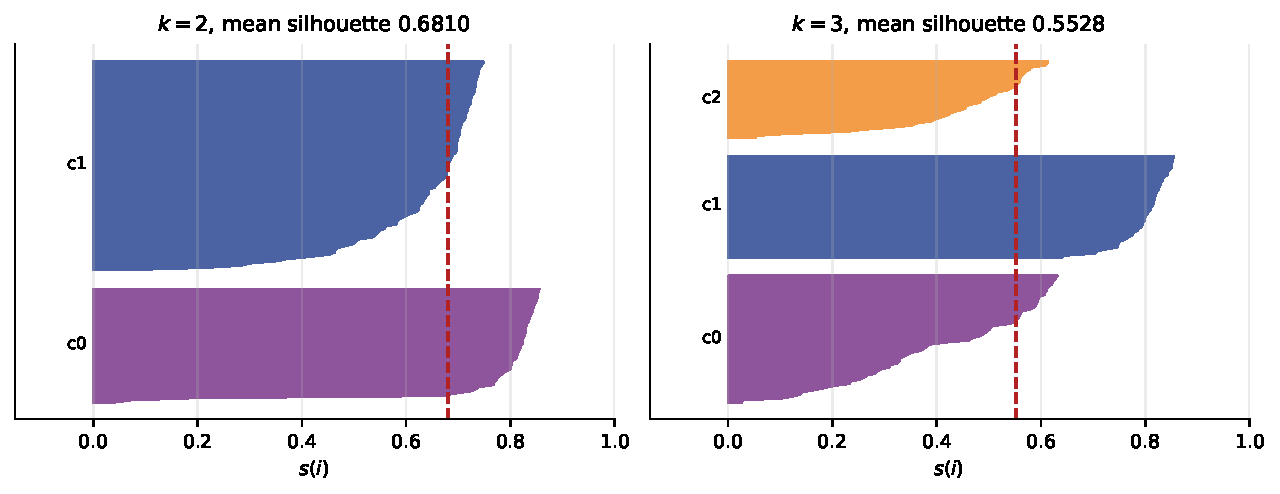
\includegraphics[width=\textwidth]{silprofile.pdf}
  \caption{The silhouette profile: every point's $s(i)$, sorted within its
  cluster, with the overall mean as a dashed line. A cluster whose bars fall
  well below the mean line is the one to investigate.}
  \label{fig:silprofile}
\end{figure}

\begin{keyidea}
Plot the profile, not just the average. A silhouette score of $0.55$ can mean
``three mediocre clusters'' or ``one excellent cluster and two poor ones'',
and the action you should take is different in the two cases.
\end{keyidea}

\subsection{Davies--Bouldin}

The third internal index in common use:
\begin{equation}
  \mathrm{DB} = \frac{1}{k}\sum_{j=1}^{k}\
    \max_{l \neq j}\ \frac{S_j + S_l}{d(c_j, c_l)},
  \qquad
  S_j = \frac{1}{n_j}\sum_{x \in C_j} \lVert x - c_j \rVert .
  \label{eq:db}
\end{equation}
$S_j$ is the average distance from the members of a cluster to its own
centroid --- its spread. For each cluster you find its \emph{worst} neighbour,
the one whose combined spread is largest relative to the distance between the
centroids, and you average those worst cases. \textbf{Lower is better}, and
zero is unattainable.

\begin{worked}[DB on the six points, clustering A]
Cluster $1$ has centroid $(3,3)$ and its members lie at distances
$\sqrt{2} = 1.414214$, $\sqrt{2} = 1.414214$ and $2$, so
\[
  S_1 = \frac{1.414214 + 1.414214 + 2}{3} = \frac{4.828427}{3} = 1.609476 .
\]
Cluster $2$ is a translate of cluster $1$, so $S_2 = 1.609476$ as well. The
centroids are $(3,3)$ and $(10,4)$, a distance $\sqrt{50} = 7.071068$ apart.
With only two clusters, each has exactly one neighbour, so
\[
  \mathrm{DB} = \frac{1}{2}\left(\frac{S_1 + S_2}{7.071068}
              + \frac{S_2 + S_1}{7.071068}\right)
              = \frac{3.218951}{7.071068} = \mathbf{0.455228},
\]
which is what \texttt{davies\_bouldin\_score} returns. Clustering B scores
$2.358045$ --- more than five times worse.
\end{worked}

The three indices measure related but genuinely different things. The
silhouette works on \textbf{pairwise distances}; Calinski--Harabasz works on
the \textbf{scatter decomposition}; Davies--Bouldin works on
\textbf{centroid spreads and centroid separations}. There is no reason for
three different summaries of a partition to rank two partitions the same way,
and they do not.

\subsection{All three across $k$, with no labels used}
\label{sec:allthree}

\begin{lstlisting}
for k in range(2, 9):
    lab = KMeans(n_clusters=k, n_init=10, random_state=0).fit_predict(X)
    print(k, silhouette_score(X, lab), calinski_harabasz_score(X, lab),
             davies_bouldin_score(X, lab))
\end{lstlisting}
\begin{codeout}
  k   silhouette           CH           DB |        ARI        NMI
  2       0.6810       513.92       0.4043 |     0.5399     0.6565
  3       0.5528       561.63       0.6620 |     0.7302     0.7582
  4       0.4981       530.77       0.7803 |     0.6498     0.7219
  5       0.4887       495.54       0.8060 |     0.6079     0.6939
  6       0.3648       473.85       0.9142 |     0.4475     0.6380
  7       0.3569       447.96       0.9628 |     0.4813     0.6689
  8       0.3597       439.46       0.9266 |     0.4570     0.6581
\end{codeout}
\begin{codeout}
silhouette prefers k = 2  (higher is better)
Calinski-Harabasz  k = 3  (higher is better)
Davies-Bouldin     k = 2  (lower  is better)
the labels prefer  k = 3  (ARI, higher is better)
two of the three internal indices disagree with the labels
\end{codeout}

\begin{figure}[htbp]
  \centering
  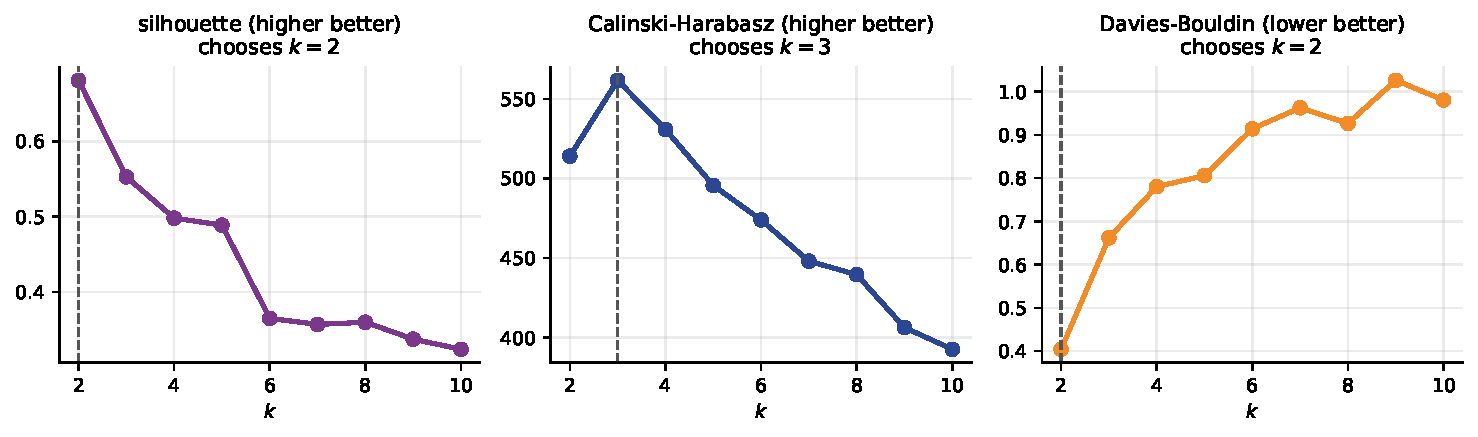
\includegraphics[width=\textwidth]{internal.pdf}
  \caption{Three internal indices on iris, all computed with no access to the
  species column. They do not agree on $k$.}
  \label{fig:internal}
\end{figure}

\subsection{External validation: ARI and NMI}
\label{sec:external}

An external index compares two \emph{partitions} of the same objects --- your
clustering and the known grouping. It must be invariant to how the clusters
are named, because cluster $0$ is not class $0$; it is just the first group
the algorithm happened to build.

\begin{lstlisting}
lab3 = KMeans(n_clusters=3, n_init=10, random_state=0).fit_predict(X)
perm = np.array([{0: 2, 1: 0, 2: 1}[v] for v in lab3])   # rename only
print(adjusted_rand_score(y, lab3), adjusted_rand_score(y, perm))
\end{lstlisting}
\begin{codeout}
relabelling the clusters 0->2, 1->0, 2->1 changes nothing:
   ARI before 0.730238   after 0.730238
   NMI before 0.758176   after 0.758176
cluster identifiers are names, not classes
\end{codeout}

\begin{caution}[\texttt{accuracy\_score(y, clusters)} is meaningless]
It compares label \emph{values}, and cluster label values are arbitrary. The
same partition can score $0.9$ or $0.0$ depending on which permutation the
algorithm happened to return. Use ARI, NMI or an explicitly matched measure;
never accuracy.
\end{caution}

The \textbf{Rand index} counts the point \emph{pairs} the two partitions agree
about --- pairs together in both, or apart in both --- divided by
$\binom{n}{2}$. That is permutation-invariant, but it has a serious defect.

\begin{lstlisting}
rng = np.random.default_rng(0)
for _ in range(200):
    r = rng.integers(0, 3, len(y))
    ri.append(rand_score(y, r)); ari_.append(adjusted_rand_score(y, r))
\end{lstlisting}
\begin{codeout}
200 completely random 3-way labellings of iris
   Rand index                   mean +0.5567  sd 0.0035
   adjusted Rand index          mean -0.0010  sd 0.0073
   normalised mutual info       mean +0.0114  sd 0.0067
\end{codeout}

A clustering produced by rolling a die scores $\mathbf{0.5567}$ on the Rand
index. The reason is that most pairs of points are in \emph{different} groups
under both partitions, and the Rand index counts those as agreements. With
$k = 3$ and roughly equal groups, about $2/3$ of pairs are apart under each
partition by chance alone.

The \textbf{adjusted Rand index} fixes this by subtracting the expected value
under a random labelling and rescaling so that the maximum is $1$:
\begin{equation}
  \mathrm{ARI} = \frac{\mathrm{RI} - \mathbb{E}[\mathrm{RI}]}
                      {\max(\mathrm{RI}) - \mathbb{E}[\mathrm{RI}]} .
  \label{eq:ari}
\end{equation}
It scores $\mathbf{-0.0010}$ on the same random labellings --- zero, to within
sampling noise --- and it can go negative, which means ``worse than chance''.

\textbf{Normalised mutual information} takes a different route. Treat the
cluster assignment and the true label as two discrete random variables and
compute their mutual information $I(U;V)$, then normalise by the entropies:
$\mathrm{NMI} = I(U;V)/\sqrt{H(U)H(V)}$ in scikit-learn's default. It lies in
$[0,1]$ and is $1$ only when the two partitions determine each other. Plain
NMI is only weakly corrected for chance ($0.0114$ above, not $0$); use
\texttt{adjusted\_mutual\_info\_score} if you need a fully corrected version.

\subsection{The honest disagreement}

\begin{figure}[htbp]
  \centering
  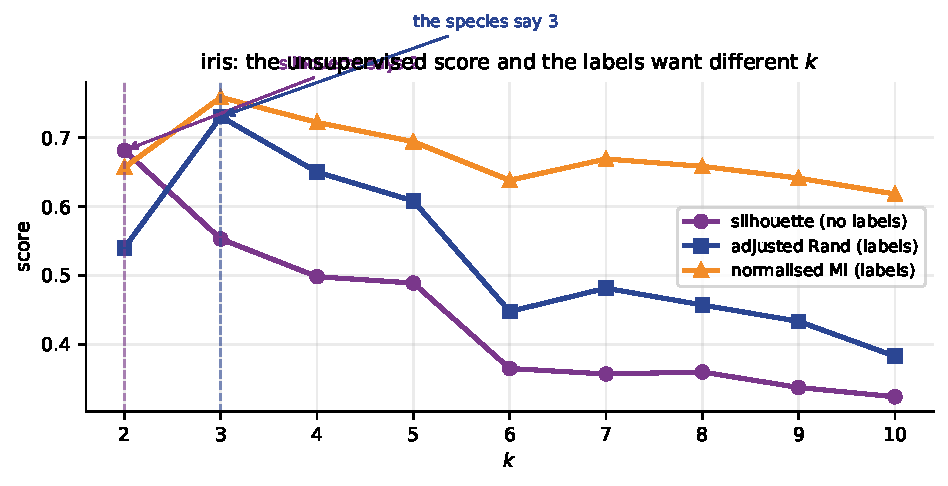
\includegraphics[width=0.78\textwidth]{external.pdf}
  \caption{The unsupervised score and the labels want different $k$. The
  silhouette peaks at $k = 2$; the adjusted Rand index and the normalised
  mutual information both peak at $k = 3$.}
  \label{fig:external}
\end{figure}

State it plainly, because it is the most important honest result in the
lecture: \textbf{on iris, the silhouette prefers a clustering that the labels
do not.} $k = 2$ scores $0.6810$ and merges two of the three species; $k = 3$
scores only $0.5528$ and recovers them.

There are three defensible readings and you should be able to give all three.

\begin{enumerate}[leftmargin=*]
  \item \emph{The index is right and the labels are the wrong question.} In
    these four measurements, \emph{versicolor} and \emph{virginica} overlap.
    A measure of separation should say so.
  \item \emph{The labels are right and the index is limited.} Species are a
    biological fact; petal geometry is a noisy proxy for it, and no
    unsupervised measure can recover a distinction the features barely encode.
  \item \emph{Both, and the useful output is the pair.} $k = 2$ is the
    strongest \emph{geometric} structure; $k = 3$ is the strongest structure
    \emph{that corresponds to something outside the data}. Reporting both,
    with the numbers, is more informative than picking one.
\end{enumerate}

What you must not do is quote $0.6810$, call the clustering validated, and
move on. That number is the value of one index at one setting, and two other
indices and the ground truth all have something different to say.

\notesources{\AMLUnitVIISources}

% =========================================================================
\section{Clustering as a preprocessing tool}
\label{sec:prep}

Clustering is not only an end in itself. Two uses feed a supervised model, and
both are worth measuring rather than assuming.

\subsection{Cluster membership as an engineered feature}
\label{sec:feat}

Fit k-means on the training rows. Then add, to each row, either the $k$
indicator columns saying which cluster it fell into, or the $k$ distances to
the centroids. A \textbf{linear} model given those columns can fit a separate
intercept in each cluster, which makes it piecewise --- non-linear --- for the
price of $k$ extra columns and no labels.

\begin{lstlisting}
Xm, ym = make_moons(n_samples=600, noise=0.15, random_state=3)
Xtr, Xte, ytr, yte = train_test_split(Xm, ym, test_size=0.3,
                                      random_state=0, stratify=ym)
km  = KMeans(n_clusters=k, n_init=10, random_state=0).fit(Xtr)
Otr = np.eye(k)[km.labels_];  Ote = np.eye(k)[km.predict(Xte)]
LogisticRegression(max_iter=5000).fit(np.hstack([Xtr, Otr]), ytr)
\end{lstlisting}
\begin{codeout}
logistic regression on the two raw columns   0.9056
    k      + one-hot    + distances
    2         0.9444         0.9667
    4         0.9722         0.9167
    6         0.9889         0.9778
    8         0.9944         0.9833
   10         0.9944         0.9833
   15         0.9944         0.9889
   20         0.9889         0.9889
\end{codeout}

From $0.9056$ to $\mathbf{0.9944}$: a model that could only draw a straight
line now follows a curved boundary, and the eight regions it uses were built
without looking at a single label.

\begin{figure}[htbp]
  \centering
  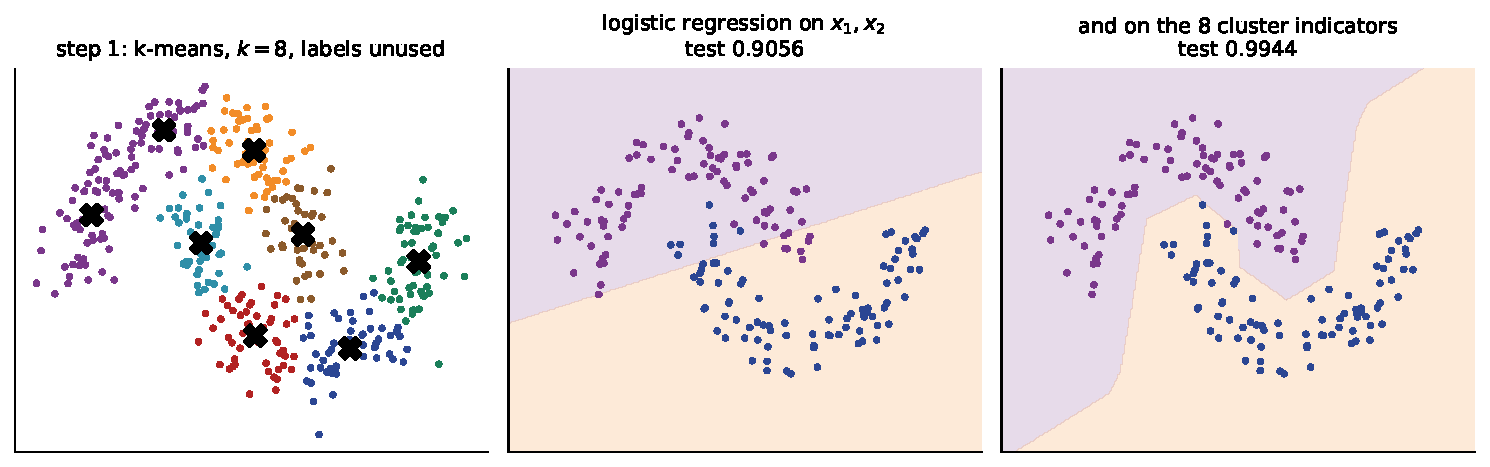
\includegraphics[width=\textwidth]{features.pdf}
  \caption{Left: k-means with $k=8$ on the training rows, labels hidden.
  Middle: logistic regression on the two coordinates draws a line. Right: the
  same model with eight cluster indicator columns added follows the cluster
  edges.}
  \label{fig:features}
\end{figure}

\subsection{And the null result, reported as it happened}

The same recipe on \texttt{load\_breast\_cancer}:

\begin{codeout}
logistic regression on the 30 scaled columns  0.9591
   +  2 cluster distances                     0.9532
   +  5 cluster distances                     0.9591
   + 10 cluster distances                     0.9649
   + 20 cluster distances                     0.9591
report the null result: on this table it buys essentially nothing
\end{codeout}

The best of the four settings gains $+0.0058$, which on $171$ test rows is
\textbf{one patient}. Two of the four made things worse. This is not a result;
it is noise, and reporting it as a $0.6$ percentage point improvement would be
dishonest.

Why the difference? The trick pays when the decision boundary is non-linear
\emph{and} the clusters happen to line up with it. On the moons both hold. On
breast cancer the thirty standardised columns are already close to linearly
separable, so there is no curvature for the extra columns to supply.

\begin{keyidea}
``Add cluster features'' is a hypothesis about your data, not a technique that
always helps. Measure the baseline, measure the augmented model, and report
whichever way it came out.
\end{keyidea}

\subsection{Cluster-then-label: spending a labelling budget}
\label{sec:budget}

Rows are usually cheap and labels are usually expensive --- a radiologist's
time, a lawyer's reading, a chemist's assay. Suppose you can afford $50$
labels out of $1257$ handwritten digits. How should you choose which $50$?

The naive answer is to pick $50$ rows at random. The better answer uses
clustering: run k-means with $k = 50$, and label the one row \emph{closest to
each centroid}. Those $50$ rows are, by construction, spread across the whole
data and each is typical of its neighbourhood. Then go one step further and
\textbf{propagate} each label to every row in its cluster, which turns $50$
labels into $1257$ approximate ones.

\begin{lstlisting}
km  = KMeans(n_clusters=B, n_init=10, random_state=0).fit(Xtr)
rep = np.argmin(km.transform(Xtr), axis=0)     # nearest row to each centroid
yprop = np.empty(len(Xtr), dtype=int)
for i in range(B): yprop[km.labels_ == i] = ytr[rep[i]]
LogisticRegression(max_iter=5000).fit(Xtr, yprop)
\end{lstlisting}
\begin{codeout}
fully supervised baseline (1257 labels) 0.9722
 budget     random       sd   representative    propagated
     10     0.4744   0.0180           0.7926        0.7741
     20     0.6378   0.0337           0.8463        0.9000
     30     0.7219   0.0374           0.9056        0.9111
     50     0.8104   0.0274           0.8981        0.9389
    100     0.8907   0.0184           0.9370        0.9370
\end{codeout}

At a budget of $50$: random selection gives $0.8104$, representative selection
$0.8981$, and propagation $\mathbf{0.9389}$ --- against $0.9722$ for labelling
everything. \textbf{Ninety-six per cent of the achievable accuracy for four
per cent of the labelling cost.} At a budget of $10$ the gap is even starker:
$0.4744$ against $0.7926$.

\begin{figure}[htbp]
  \centering
  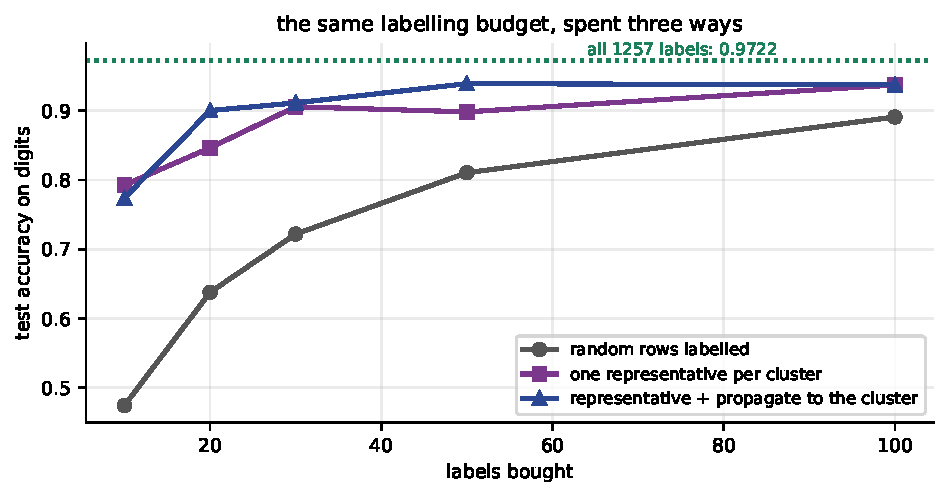
\includegraphics[width=0.78\textwidth]{budget.pdf}
  \caption{The same labelling budget spent three ways on \texttt{load\_digits}.
  Random selection is the grey line; the dotted line is what all $1257$ labels
  achieve.}
  \label{fig:budget}
\end{figure}

Propagation clearly introduces errors, so it is worth measuring how many.

\begin{codeout}
50 labels bought; 1257 training rows labelled by propagation
propagated labels that are actually correct: 1206 of 1257 (0.9594)
so the cheap model trains on 4.06% wrong labels
\end{codeout}

Fifty-one of the $1257$ propagated labels are wrong. The model still wins,
because logistic regression tolerates $4\%$ label noise far better than it
tolerates having only $50$ training rows. That trade --- a little noise for a
lot of data --- is the whole idea.

\subsection{The leakage rule}
\label{sec:leak}

\begin{caution}[Fit the clusterer on the training rows only]
Both techniques above fit k-means on \texttt{Xtr} and then call
\texttt{predict} on \texttt{Xte}. If you fit k-means on the whole dataset
before splitting, the centroids --- and therefore the engineered features ---
have been computed using the test rows, and your test score is optimistic.

This is the same rule you met for \texttt{StandardScaler}, in a new costume.
The general form is: \textbf{any object with a \texttt{fit} method must be fit
inside the training fold.} Inside a \texttt{Pipeline} and
\texttt{cross\_val\_score}, scikit-learn enforces this for you, which is the
main reason to use them.
\end{caution}

There is a related trap worth naming. Clustering is sometimes done after
dimensionality reduction, and the order matters less than people fear but not
zero:

\begin{codeout}
PCA first two components explain 0.9777 of the variance
cluster in 4D then project : ARI vs labels 0.7302
project to 2D then cluster : ARI vs labels 0.7163
the two clusterings agree with each other : ARI 0.9803
\end{codeout}

On iris the two orders agree at ARI $0.9803$ and differ by $0.0139$ against
the species --- because two components already carry $97.77\%$ of the
variance. On a dataset where they carry $60\%$, the two orders can differ a
great deal. Decide deliberately, and say which you did.

\notesources{\AMLUnitVIISources}

% =========================================================================
\section{General applications of clustering}
\label{sec:apps}

Four families of use, kept concrete.

\textbf{Segmentation.} Customers grouped by purchase behaviour, so a campaign
can be written for each group instead of for an average customer nobody
resembles. Students grouped by attempt patterns, so that the right
intervention reaches the right group. The cluster here corresponds to
\emph{a population you will treat differently}, and the test of the clustering
is whether treating them differently works.

\textbf{Organising a corpus.} Documents grouped into topics for browsing;
search results grouped so that a query with two meanings returns two piles;
genes grouped by correlated expression profiles, which is how co-regulated
gene sets were first found. The cluster corresponds to \emph{a heading in a
table of contents that nobody wrote}.

\textbf{Compression and summarisation.} Vector quantisation: replace every
value by its cluster centre, and store the small codebook plus one index per
item. Colour palettes are the textbook case.

\begin{codeout}
image 427 x 640 pixels, 96615 distinct colours
   k=  2  palette   2 colours  MSE 0.019764  storage  4.17% of 24-bit
   k=  4  palette   4 colours  MSE 0.007028  storage  8.34% of 24-bit
   k=  8  palette   8 colours  MSE 0.003246  storage 12.51% of 24-bit
   k= 16  palette  16 colours  MSE 0.001792  storage 16.69% of 24-bit
   k= 32  palette  32 colours  MSE 0.000998  storage 20.88% of 24-bit
\end{codeout}

Sixteen colours in place of $96\,615$ reproduces the image at a mean squared
error of $0.0018$ per channel, in about a sixth of the storage. The cluster
corresponds to \emph{an entry in a codebook}.

\begin{figure}[htbp]
  \centering
  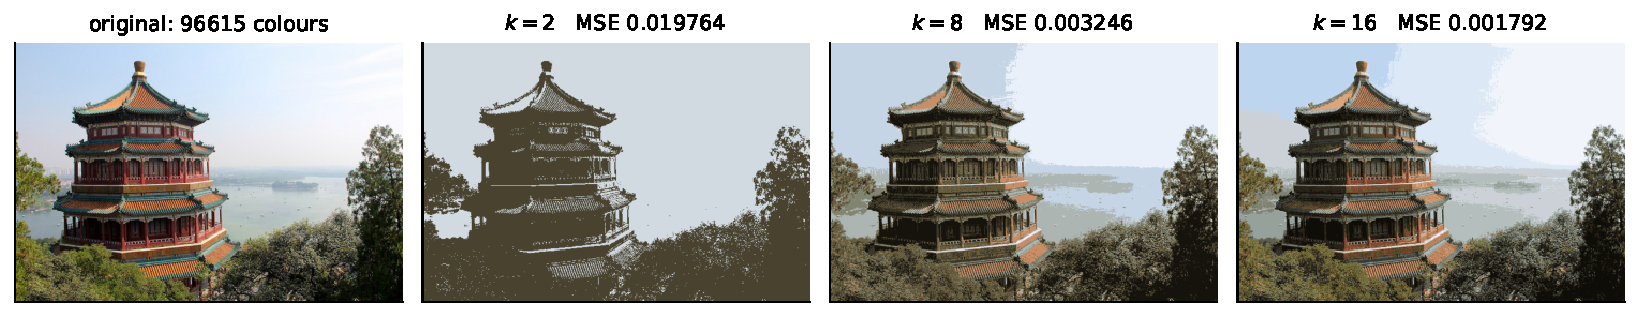
\includegraphics[width=\textwidth]{quantise.pdf}
  \caption{Colour quantisation. Each pixel is a point in $\mathbb{R}^3$;
  k-means finds a palette; every pixel is replaced by its centroid.}
  \label{fig:quantise}
\end{figure}

\textbf{Anomaly detection.} Points that fall in no cluster, or in a cluster of
size one, are candidates for fraudulent transactions, network intrusions or
faulty sensors. Density-based methods hand you this for free, since they
already refuse to assign some points. Measured on the moons with twelve
uniform outliers planted:

\begin{lstlisting}
rng = np.random.default_rng(0)               # the one seed for this lecture
Xm, _ = make_moons(n_samples=500, noise=0.06, random_state=7)
out = rng.uniform([-1.5, -1.0], [2.5, 1.5], size=(12, 2))
lab = DBSCAN(eps=0.20, min_samples=5).fit_predict(np.vstack([Xm, out]))
\end{lstlisting}
\begin{codeout}
500 structured points + 12 uniform outliers
   DBSCAN flagged 8 points as noise
   of those, 8 are planted outliers and 0 are structured points
   recall on the planted outliers 0.6667, precision 1.0000
\end{codeout}

Report that as it is: \textbf{precision $1.0000$, recall $0.6667$}. Every
point DBSCAN flagged really was an outlier, but it missed a third of them,
because four of the twelve landed inside or against the crescents where
the local density is perfectly ordinary. That is the honest limit of the
technique: \emph{it detects points in sparse regions, which is not the same
thing as points that do not belong}.

Finally, a use that is really a demonstration. Run k-means with $k = 10$ on
$1797$ digit images with the labels hidden:

\begin{codeout}
k-means with k=10 on 1797 unlabelled digit images
   ARI vs the true digit 0.6657, NMI 0.7425
   cluster : dominant digit (purity)
      0 : 0 (176 of 178 = 0.99)      5 : 6 (177 of 182 = 0.97)
      1 : 1 (100 of 223 = 0.45)      6 : 4 (165 of 169 = 0.98)
      2 : 7 (174 of 208 = 0.84)      7 : 5 (136 of 150 = 0.91)
      3 : 1 ( 54 of  87 = 0.62)      8 : 9 (139 of 247 = 0.56)
      4 : 3 (154 of 178 = 0.87)      9 : 2 (148 of 175 = 0.85)
   overall purity 0.7919
\end{codeout}

Knowing nothing but $64$ pixel values, the algorithm produces groups that are
$79\%$ pure. Zeros, sixes and fours come out almost perfectly. The failures
are the interesting part: \textbf{ones are split across two clusters} (0.45
and 0.62 pure), and nines and eights are muddled --- which is roughly what a
human misreads too.

\begin{caution}[Purity is not an honest index on its own]
Purity always increases as $k$ increases, and reaches $1$ at $k = n$. It is
readable and it is useful alongside a confusion table, but it is in the same
family as $W$: monotone in $k$, and therefore useless for choosing $k$. Quote
ARI or NMI beside it.
\end{caution}

\notesources{\AMLUnitVIISources}

% =========================================================================
\section{Summary}
\label{sec:summary}

\begin{enumerate}[leftmargin=*]
  \item Clustering divides objects into groups so that within-group objects
    are similar and between-group objects are not. There is \textbf{no target
    column}, so the objective is a modelling choice and validation must be
    rebuilt from geometry.
  \item \textbf{There is no single right answer.} On iris the silhouette
    prefers $k = 2$ ($0.6810$ against $0.5528$) while the species prefer
    $k = 3$ (ARI $0.7302$ against $0.5399$); the two clusterings agree with
    each other at ARI only $\mathbf{0.5516}$.
  \item Feature scaling \emph{is} the definition of similarity. On wine, raw
    against standardised gives ARI to the cultivar of $0.3711$ and
    $\mathbf{0.8975}$, and the two clusterings agree at $0.3543$ --- because
    \texttt{proline} carries $99.77\%$ of the raw variance.
  \item Five families: \textbf{partitioning, hierarchical, density-based,
    grid-based, model-based}, distinguished by what they assume a cluster
    looks like.
  \item Those assumptions have consequences. On two moons k-means scores
    $\mathbf{0.2445}$ and DBSCAN $\mathbf{1.0000}$; on elongated blobs
    k-means scores $0.5554$ and a Gaussian mixture $1.0000$; on unequal
    spread single linkage scores $\mathbf{0.0002}$. \textbf{No algorithm wins
    all four datasets.}
  \item A grid clusterer is a histogram plus a flood fill: $43$ dense cells of
    $100$, two components, ARI $0.9643$ --- and at $\tau = 2$, $G = 12$ the
    arms bridge and it collapses to $\mathbf{0.0000}$.
  \item Centroid $c_j = \frac{1}{n_j}\sum_{x \in C_j} x$; it minimises the sum
    of squared distances to its members, and that single fact proves
    everything else.
  \item \textbf{$T = W + B$.} On six points, $91 = 16 + 75$ for one clustering
    and $91 = 79 + 12$ for another. On iris, $T = 681.370600$ at every $k$
    with residual at most $1.14 \times 10^{-13}$.
  \item Since $T$ is fixed, \textbf{minimising $W$ and maximising $B$ are one
    problem}. $W$ falls monotonically to $0$ at $k = n$, so it cannot choose
    $k$; the elbow is a visual heuristic on a curve with no optimum.
  \item $\mathrm{CH} = \frac{B/(k-1)}{W/(n-k)}$ restores the penalty:
    $75/4 = \mathbf{18.75}$ by hand, $18.7500$ from scikit-learn.
  \item Silhouette $s(i) = (b - a)/\max(a,b)$. By hand $s(P_1) =
    \mathbf{0.691137}$; the mean over the six is $0.618068$, and the rival
    clustering scores $\mathbf{-0.071164}$ --- negative means misassigned.
    Davies--Bouldin on the same clustering is $0.455228$ by hand.
  \item Internal indices disagree with each other: on iris, silhouette says
    $k=2$, Calinski--Harabasz says $k=3$, Davies--Bouldin says $k=2$.
    \textbf{Report the ones that disagree with you.}
  \item External measures must be chance-corrected: a random 3-way labelling
    of iris scores Rand $\mathbf{0.5567}$ but ARI $\mathbf{-0.0010}$.
    Renaming clusters changes neither ARI nor NMI, so plain accuracy
    against cluster labels is undefined.
  \item As preprocessing it works when it works: moons
    $0.9056 \to \mathbf{0.9944}$ with eight cluster indicators, but
    \texttt{breast\_cancer} $0.9591 \to 0.9649$, which is one patient.
  \item Cluster-then-label reaches $\mathbf{0.9389}$ on $50$ labels against
    $0.8104$ spent at random and $0.9722$ for all $1257$, at the cost of
    $4.06\%$ wrong propagated labels.
  \item Applications: segmentation, corpus organisation, vector quantisation
    ($96\,615$ colours to $16$ at MSE $0.0018$), and anomaly detection
    (precision $1.0000$, recall $0.6667$ on planted outliers).
\end{enumerate}

% =========================================================================
\section{Practice questions}
\label{sec:practice}

Work these with a pen before looking at Section~\ref{sec:solutions}.
Questions 1, 2 and 5 are pure hand arithmetic and are the kind most likely to
appear in a written paper.

\begin{enumerate}[leftmargin=*]
  \item \textbf{(Centroids, $W$, $B$, $T$ by hand.)} Take the six points
    $P_1(2,2)$, $P_2(4,2)$, $P_3(3,5)$, $P_4(9,3)$, $P_5(11,3)$, $P_6(10,6)$
    and the clustering $\mathcal{C} = \{\{P_1,P_2,P_3,P_4\},\{P_5,P_6\}\}$.
    Compute both centroids, then $W$, $B$ and $T$, and verify $T = W + B$.
    Compare $W$ with the value $16$ obtained for clustering A in
    Section~\ref{sec:byhand} and say which clustering k-means would prefer.

  \item \textbf{(Silhouette by hand, including a negative one.)} Using the
    distance matrix printed in Section~\ref{sec:silhand} and the clustering
    $\mathcal{C}$ of Question 1, compute $a(P_4)$, $b(P_4)$ and $s(P_4)$.
    Interpret the sign of your answer in one sentence.

  \item \textbf{(Calinski--Harabasz.)} For the clustering $\mathcal{C}$ of
    Question 1, compute $\mathrm{CH}$. Then explain, in two sentences, why
    dividing $B$ by $k-1$ prevents the index from being maximised at $k = n$.

  \item \textbf{(Why $W$ is monotone.)} Prove that splitting one cluster into
    two non-empty parts cannot increase $W$. You may use
    equation~\eqref{eq:shift}. What does your proof imply about ``choose the
    $k$ that minimises $W$''?

  \item \textbf{(Davies--Bouldin by hand.)} Two clusters have centroids
    $(0,0)$ and $(6,8)$, with average member-to-centroid distances
    $S_1 = 1.5$ and $S_2 = 2.5$. Compute the Davies--Bouldin index. If a
    third cluster were added at $(3,4)$ with $S_3 = 3.0$, would you expect DB
    to rise or fall? Why?

  \item \textbf{(Chance correction.)} A colleague reports that their
    clustering of $150$ items into $3$ groups achieves a Rand index of
    $0.56$ against a known grouping, and describes this as ``moderate
    agreement''. What is wrong with the claim, what number should they have
    reported, and roughly what would it be?

  \item \textbf{(Choosing a family.)} For each of the following, name the
    family of clustering algorithm you would try first and give the shape
    assumption that justifies it. (a) Customers described by ten
    standardised spending features, expected to form a few broad groups of
    similar size. (b) GPS pings from delivery riders, where the interesting
    structure is roads and there is a lot of stray noise. (c) A dataset where
    you believe each group is an elongated ellipse at a different angle.
    (d) Two billion records, where you can afford one pass over the data.

  \item \textbf{(Scaling.)} On wine, clustering the raw table gives ARI
    $0.3711$ against the cultivar and clustering the standardised table gives
    $0.8975$. A student concludes ``therefore you should always
    standardise before clustering''. Give one situation where that advice is
    wrong, and state the general principle it should be replaced by.

  \item \textbf{(Cluster-then-label.)} With a budget of $50$ labels on
    \texttt{load\_digits}, propagation reached $0.9389$ while training only on
    the $50$ representatives reached $0.8981$ --- even though propagation
    introduces $51$ wrong labels. Explain the mechanism. Then say what you
    would expect to happen to the propagation result if the $50$ clusters were
    replaced by $5$.

  \item \textbf{(Leakage and reporting.)} A report says: ``We ran k-means on
    the full dataset, added the cluster identity as a feature, split the data
    $70/30$, and improved test accuracy from $0.951$ to $0.958$.'' Identify
    two separate problems with this sentence, and say what you would need to
    see before believing the improvement.
\end{enumerate}

% =========================================================================
\section{Solutions}
\label{sec:solutions}

\subsection*{Solution 1 --- centroids, $W$, $B$, $T$}

\textbf{Centroids.} For $\{P_1,P_2,P_3,P_4\}$:
\[
  c_1 = \Bigl(\tfrac{2+4+3+9}{4},\ \tfrac{2+2+5+3}{4}\Bigr)
      = \Bigl(\tfrac{18}{4},\ \tfrac{12}{4}\Bigr) = (4.5,\ 3.0).
\]
For $\{P_5,P_6\}$:
\[
  c_2 = \Bigl(\tfrac{11+10}{2},\ \tfrac{3+6}{2}\Bigr) = (10.5,\ 4.5).
\]

\textbf{Within.} Offsets from $c_1 = (4.5,3)$:
\begin{center}
\begin{tabular}{@{}lll@{}}
  \toprule
  point & offset & squared length \\
  \midrule
  $P_1(2,2)$  & $(-2.5,\,-1.0)$ & $6.25 + 1.00 = 7.25$ \\
  $P_2(4,2)$  & $(-0.5,\,-1.0)$ & $0.25 + 1.00 = 1.25$ \\
  $P_3(3,5)$  & $(-1.5,\,+2.0)$ & $2.25 + 4.00 = 6.25$ \\
  $P_4(9,3)$  & $(+4.5,\,\ 0.0)$ & $20.25 + 0.00 = 20.25$ \\
  \bottomrule
\end{tabular}
\end{center}
so the first cluster contributes $7.25 + 1.25 + 6.25 + 20.25 = 35$. Offsets
from $c_2 = (10.5,4.5)$ are $(0.5,-1.5)$ and $(-0.5,1.5)$, each of squared
length $0.25 + 2.25 = 2.5$, contributing $5$. Hence
\[
  W = 35 + 5 = \mathbf{40}.
\]

\textbf{Between.} The grand mean is $(6.5, 3.5)$.
\[
  \lVert (4.5,3.0)-(6.5,3.5)\rVert^2 = 4 + 0.25 = 4.25,
  \qquad
  \lVert (10.5,4.5)-(6.5,3.5)\rVert^2 = 16 + 1 = 17,
\]
\[
  B = 4(4.25) + 2(17) = 17 + 34 = \mathbf{51}.
\]

\textbf{Total.} $T = 91$, unchanged --- it depends only on the points and the
grand mean, both of which are the same as in Section~\ref{sec:byhand}. And
$40 + 51 = 91$. \checkmark

\textbf{Which does k-means prefer?} k-means minimises $W$, and
$16 < 40$, so it prefers clustering A. Running it confirms this: it returns
clustering A with \texttt{inertia\_} $= 16.0000$.

\begin{codeout}
C centroids [4.5 3. ] [10.5  4.5]
C: T 91.0000 W 40.0000 B 51.0000  sum 91.0000
\end{codeout}

\subsection*{Solution 2 --- silhouette of $P_4$ under $\mathcal{C}$}

$P_4$ now sits in the \emph{first} cluster, $\{P_1,P_2,P_3,P_4\}$, so
\[
  a(P_4) = \frac{d(P_4,P_1) + d(P_4,P_2) + d(P_4,P_3)}{3}
         = \frac{7.0711 + 5.0990 + 6.3246}{3}
         = \frac{18.4947}{3} = 6.164881 .
\]
The only other cluster is $\{P_5,P_6\}$, so
\[
  b(P_4) = \frac{d(P_4,P_5) + d(P_4,P_6)}{2}
         = \frac{2.0000 + 3.1623}{2} = \frac{5.1623}{2} = 2.581139 .
\]
Here $a > b$, so the denominator is $a$:
\[
  s(P_4) = \frac{b - a}{\max\{a,b\}} = \frac{2.581139 - 6.164881}{6.164881}
         = \frac{-3.583742}{6.164881} = \mathbf{-0.581316}.
\]

\textbf{Interpretation.} The value is negative, which means $P_4$ is on
average much closer to the members of the other cluster than to its own
cluster-mates --- it has been put in the wrong group, and moving it to
$\{P_5,P_6\}$ would improve the clustering. That is exactly right: $P_4(9,3)$
belongs geometrically with $P_5$ and $P_6$ on the right, not with the three
points on the left.

\begin{codeout}
C per-point [ 0.546904  0.521021  0.449462 -0.581316  0.52037   0.520662]
C silhouette 0.329517
\end{codeout}

\subsection*{Solution 3 --- Calinski--Harabasz}

With $B = 51$, $W = 40$, $k = 2$, $n = 6$:
\[
  \mathrm{CH} = \frac{51/(2-1)}{40/(6-2)} = \frac{51}{10} = \mathbf{5.10},
\]
against $18.75$ for clustering A --- so CH agrees with $W$ and with the
silhouette that A is much better.

\textbf{Why the $k-1$ matters.} As $k$ grows towards $n$, $B$ grows towards
$T$ and $W$ shrinks towards $0$, so the raw ratio $B/W$ diverges and would
always select $k = n$. Dividing $B$ by $k-1$ charges a growing price for each
additional cluster, and dividing $W$ by $n-k$ inflates the denominator's
per-degree-of-freedom size as $k$ grows; together they turn a monotone
quantity into one with an interior maximum.

\subsection*{Solution 4 --- $W$ is monotone in $k$}

Let cluster $C$ with centroid $c$ be split into non-empty parts $C'$ and
$C''$ with centroids $c'$ and $c''$. Its contribution to $W$ before the split
is $\sum_{x \in C}\lVert x - c\rVert^2$. Apply equation~\eqref{eq:shift}
separately to each part, taking $m = c$:
\[
  \sum_{x \in C'}\lVert x - c\rVert^2
    = \sum_{x \in C'}\lVert x - c'\rVert^2 + |C'|\,\lVert c' - c\rVert^2
  \ \geq\ \sum_{x \in C'}\lVert x - c'\rVert^2 ,
\]
and likewise for $C''$. Adding the two and noting that the left sides sum to
the pre-split contribution:
\[
  \sum_{x \in C}\lVert x - c\rVert^2
  \ \geq\ \sum_{x \in C'}\lVert x - c'\rVert^2
        + \sum_{x \in C''}\lVert x - c''\rVert^2 ,
\]
which is the post-split contribution. Every other cluster is untouched, so
$W$ cannot increase. Equality holds only if $c' = c'' = c$. \ensuremath{\square}

\textbf{Implication.} ``Choose the $k$ minimising $W$'' always returns
$k = n$, where every point is its own cluster and $W = 0$. $W$ is a measure of
fit, not a model-selection criterion; any procedure that selects $k$ must add
a penalty for $k$ (as Calinski--Harabasz does) or use a different quantity
entirely (as the silhouette does).

\subsection*{Solution 5 --- Davies--Bouldin}

The centroid distance is $d = \sqrt{6^2 + 8^2} = \sqrt{100} = 10$. With two
clusters each has exactly one candidate neighbour, so the maximum in
equation~\eqref{eq:db} is over a single term for each:
\[
  R_{12} = R_{21} = \frac{S_1 + S_2}{d} = \frac{1.5 + 2.5}{10} = 0.4,
  \qquad
  \mathrm{DB} = \tfrac{1}{2}(0.4 + 0.4) = \mathbf{0.40}.
\]

\textbf{Adding a third cluster at $(3,4)$.} DB would \emph{rise} (get worse).
That point is the midpoint of the segment joining the two centroids, at
distance $5$ from each, and it has the largest spread of the three
($S_3 = 3.0$). Its ratios against both neighbours are
$(1.5+3.0)/5 = 0.90$ and $(2.5+3.0)/5 = 1.10$, so cluster $3$ contributes
$\max = 1.10$; clusters $1$ and $2$ now also have a close, wide neighbour and
their worst-case ratios rise to $0.90$ and $1.10$. The average is
$(0.90 + 1.10 + 1.10)/3 = 1.0\overline{3}$, well above $0.40$. The general
lesson: DB punishes a cluster that is both wide and close to another one, and
inserting a wide cluster between two tight ones is the worst case for it.

\subsection*{Solution 6 --- chance correction}

\textbf{What is wrong.} The Rand index is not corrected for chance. On $150$
items in $3$ groups, a completely random labelling scores about $0.5567$ on
average --- so $0.56$ is what you get from rolling a die, and it is evidence
of nothing whatever. Describing it as ``moderate agreement'' is describing
noise.

\textbf{What to report.} The \textbf{adjusted} Rand index, which subtracts the
expected value under random labelling and rescales so that the maximum is $1$:
$\mathrm{ARI} = (\mathrm{RI} - \mathbb{E}[\mathrm{RI}]) /
(\max \mathrm{RI} - \mathbb{E}[\mathrm{RI}])$.

\textbf{Roughly what value?} Since the reported RI is essentially the chance
value, the ARI would be approximately $\mathbf{0}$ --- the measured mean over
$200$ random labellings of iris was $-0.0010$ with standard deviation
$0.0073$, so anything in roughly $[-0.02, +0.02]$ is indistinguishable from
chance. Normalised mutual information would likewise be near $0.01$, not $0.5$.

\subsection*{Solution 7 --- choosing a family}

\textbf{(a) Partitioning (k-means).} The features are standardised, the groups
are expected to be broad and of similar size, and no unusual shape is
suggested. That is precisely the convex, roughly spherical, roughly
equal-sized assumption k-means makes, and it is fast. Start there and check
the silhouette profile.

\textbf{(b) Density-based (DBSCAN).} Roads are long thin connected structures
--- exactly the ``dense region of arbitrary shape'' that k-means cannot
represent and DBSCAN can. It also has a built-in noise category, so the stray
pings are handled rather than forced into a cluster. This is the two-moons
result in a real setting.

\textbf{(c) Model-based (a full-covariance Gaussian mixture).} An elongated
ellipse at an arbitrary angle is exactly a Gaussian with a full covariance
matrix. This is the elongated-blobs row of Section~\ref{sec:shapes}, where the
mixture scored $1.0000$ and k-means $0.5554$.

\textbf{(d) Grid-based.} The cost of a grid method is driven by the number of
cells rather than the number of points, and it needs only one pass to build
the histogram. No distance-matrix method is available at two billion records,
and even k-means needs several passes.

\subsection*{Solution 8 --- when not to standardise}

\textbf{A situation where the advice is wrong.} When the columns are already
in the same, meaningful unit and their relative magnitudes carry the
information. Pixel intensities in an image, the $64$ columns of
\texttt{load\_digits}, or the RGB values in the colour-quantisation example
are all on a common scale, and standardising them column by column would
inflate the low-variance pixels --- mostly border pixels that are almost
always blank --- into important dimensions. A second case: when you
deliberately want a high-variance column to dominate because it is the
quantity you care about.

\textbf{The principle it should be replaced by.} Scaling is not a hygiene
step, it is \textbf{the specification of what ``similar'' means}. Choose it
from the meaning of the columns: standardise when the columns are in
incomparable units and you want each to count equally; leave them alone when
they share a unit and their relative sizes are meaningful; and in either case
say which you did, because it is part of the result.

\subsection*{Solution 9 --- why propagation wins}

\textbf{The mechanism.} Training on the $50$ representatives gives a model
$50$ perfectly labelled rows. Propagation gives it $1257$ rows of which
$1206$ are correctly labelled --- $95.94\%$ accurate, so $51$ are wrong. The
model therefore trades a $4.06\%$ label-noise rate for a
$25\times$ increase in training data. For logistic regression on $64$
features, $50$ rows is severely data-starved: the estimate of each
coefficient is dominated by sampling variance. Adding a thousand more rows
reduces that variance far more than $4\%$ label noise increases the bias, so
the propagated model wins, $0.9389$ against $0.8981$.

\textbf{With $5$ clusters instead of $50$.} It would get much worse. Each
cluster would then contain roughly $250$ images spanning several digits, and
a single representative's label would be propagated to all of them, so the
propagated label accuracy would collapse from $95.94\%$ towards something
near $\tfrac{1}{5}$ of the rows. You would be training on mostly wrong labels,
and the noise term would dominate. The budget-$10$ row of the table already
shows the beginning of this effect: at $B = 10$, propagation ($0.7741$)
is \emph{worse} than the $10$ representatives alone ($0.7926$) --- the only
budget in the table where that happens.

\subsection*{Solution 10 --- leakage and reporting}

\textbf{Problem 1: leakage.} k-means was fitted on the \emph{full} dataset
before the split, so the centroids were computed using the test rows. The
engineered feature therefore encodes information about the test set, and the
reported test accuracy is optimistically biased. The fix is to split first,
fit k-means inside the training fold, and \texttt{predict} cluster identity
for the test rows --- or simply to put the clusterer and the classifier in a
\texttt{Pipeline} and let \texttt{cross\_val\_score} enforce it.

\textbf{Problem 2: the effect size is not distinguishable from noise.}
$0.951 \to 0.958$ on a single $30\%$ test split is a difference of $0.007$.
If the test set has a few hundred rows that is one or two rows, well inside
the variation you would see from changing \texttt{random\_state}. This is the
\texttt{breast\_cancer} result of Section~\ref{sec:prep} exactly: $+0.0058$,
which was one patient, and which the notes reported as a null result.

\textbf{What you would need to see.} Repeated cross-validation --- say five
repeats of five-fold --- giving a mean and a standard deviation for both the
baseline and the augmented model, with the clusterer inside the pipeline; the
number of test rows; how $k$ was chosen, and whether it was chosen on the test
set (a third leak if so); and ideally a paired test across folds rather than
two point estimates.

% =========================================================================
\section{References and further reading}
\label{sec:refs}

All links were checked on 24 August 2026. Free resources are marked
\textbf{[free]}.

\subsection*{Textbooks}

\begin{itemize}[leftmargin=*]
  \item Han, Kamber and Pei, \emph{Data Mining: Concepts and Techniques}, 3rd
    edition, Morgan Kaufmann, 2012. \textbf{The prescribed text for this
    lecture.} \S10.1 is this lecture almost exactly --- \S10.1.1 ``What is
    cluster analysis?'' and its application list, \S10.1.2 ``Requirements for
    cluster analysis'' (the checklist of scalability, arbitrary shape, noise
    tolerance and interpretability that Section~\ref{sec:tax} makes concrete),
    and \S10.1.3 ``An overview of basic clustering methods'', which is the
    five-family taxonomy in the same order used here. \S10.2 is partitioning,
    \S10.3 hierarchical, \S10.4 density-based, \S10.5 grid-based and \S10.6
    evaluation of clustering, including the chance-correction discussion of
    Section~\ref{sec:external}.
  \item M\"uller and Guido, \emph{Introduction to Machine Learning with
    Python}, O'Reilly, 2016. \textbf{Also prescribed for this lecture.}
    \S3.5 unsupervised learning: clustering --- \S3.5.1 k-means with the
    failure cases of Section~\ref{sec:shapes} drawn, \S3.5.2 agglomerative
    clustering, \S3.5.3 DBSCAN, and \textbf{\S3.5.4 ``Comparing and
    evaluating clustering algorithms''}, which is Section~\ref{sec:valid} of
    these notes: the adjusted Rand index, why accuracy must not be used, and
    silhouette scoring with its limitation on non-convex clusters. \S3.5.5
    is the summary. Notebooks \textbf{[free]}:
    \url{https://github.com/amueller/introduction_to_ml_with_python}
  \item James, Witten, Hastie, Tibshirani and Taylor, \emph{An Introduction to
    Statistical Learning with Python}. \textbf{[free]} Chapter 12 is
    unsupervised learning: \S12.1 states the ``no simple goal'' problem that
    Section~\ref{sec:noright} demonstrates, \S12.4 is clustering, \S12.4.1
    k-means with the within-cluster variation objective written exactly as
    equation~\eqref{eq:W}, \S12.4.2 hierarchical clustering and the linkage
    comparison, and \S12.4.3 ``Practical issues in clustering'' --- the
    scaling decision of Section~\ref{sec:scaling} and the warning that small
    perturbations change the answer. \url{https://www.statlearning.com/}
  \item Hastie, Tibshirani and Friedman, \emph{The Elements of Statistical
    Learning}, 2e, Springer. \textbf{[free]} \S14.3 cluster analysis: \S14.3.2
    dissimilarities, \S14.3.5 k-means with the $T = W + B$ decomposition
    stated at \S14.3.4 in the notation used here, \S14.3.8 hierarchical
    clustering, \S14.3.11 the practical difficulty of choosing $k$.
    \url{https://hastie.su.domains/ElemStatLearn/}
  \item Kaufman and Rousseeuw, \emph{Finding Groups in Data: An Introduction
    to Cluster Analysis}, Wiley, 1990. The book that introduced the silhouette
    and k-medoids. Chapter 2 is the silhouette in full, including the
    interpretation table for the average silhouette width that most
    subsequent textbooks copy.
\end{itemize}

\subsection*{Online courses}

\begin{sloppypar}
\begin{itemize}[leftmargin=*]
  \item \textbf{NPTEL, Introduction to Machine Learning} --- Prof.\ Balaraman
    Ravindran, IIT Madras; the reference course for the semester. Its
    clustering week covers partitional and hierarchical clustering in the
    notation used here. \textbf{[free]}
    \url{https://nptel.ac.in/courses/106106139}
  \item \textbf{NPTEL, Data Mining} --- Prof.\ Pabitra Mitra, IIT Kharagpur.
    Follows the Han--Kamber--Pei chapter structure, so its clustering weeks
    map directly onto \S10.1--\S10.5. \textbf{[free]}
    \url{https://nptel.ac.in/courses/106105174}
  \item \textbf{NPTEL, Introduction to Machine Learning} --- Prof.\ Sudeshna
    Sarkar, IIT Kharagpur. A second treatment of clustering worked at the
    board, if the first does not land. \textbf{[free]}
    \url{https://nptel.ac.in/courses/106105152}
  \item \textbf{SWAYAM} --- the national portal hosting NPTEL, with
    certification cycles. \textbf{[free]} \url{https://swayam.gov.in/}
  \item \textbf{Google, Introduction to Clustering} --- a short course whose
    structure is close to this lecture: ``What is clustering?'', ``Clustering
    algorithms'' (the taxonomy), ``Clustering workflow'', and ``Evaluating
    results''. \textbf{[free]}
    \url{https://developers.google.com/machine-learning/clustering}
  \item \textbf{Google Machine Learning Crash Course} --- the background for
    the supervised half of Section~\ref{sec:prep}. \textbf{[free]}
    \url{https://developers.google.com/machine-learning/crash-course}
\end{itemize}
\end{sloppypar}

\subsection*{Videos}

\begin{itemize}[leftmargin=*]
  \item StatQuest with Josh Starmer, \emph{StatQuest: K-means clustering} ---
    the assign-and-update loop drawn out at a whiteboard, with the elbow
    method at the end. Watch this one first. \textbf{[free]}
    \url{https://youtu.be/4b5d3muPQmA}
  \item StatQuest with Josh Starmer, \emph{StatQuest: Hierarchical
    Clustering} --- the dendrogram and the linkage choices, which is the
    second family in Section~\ref{sec:tax} and the subject of a later
    lecture. \textbf{[free]} \url{https://youtu.be/7xHsRkOdVwo}
  \item StatQuest with Josh Starmer, \emph{Clustering with DBSCAN, Clearly
    Explained!!!} --- core points, border points and noise, and why this
    handles the two-moons problem that k-means cannot. \textbf{[free]}
    \url{https://youtu.be/RDZUdRSDOok}
  \item Victor Lavrenko, \emph{K-means clustering: how it works} --- a slower,
    more mathematical treatment including the objective function and the
    proof that the algorithm decreases it at every step. \textbf{[free]}
    \url{https://youtu.be/_aWzGGNrcic}
\end{itemize}

\subsection*{Documentation and interactive explainers}

\begin{itemize}[leftmargin=*]
  \item scikit-learn user guide, \emph{2.3. Clustering} --- the reference for
    every estimator used here. The overview table at the top lists each
    algorithm's parameters, scalability and \textbf{``geometry (metric
    used)''}, which is the taxonomy of Section~\ref{sec:tax} in the
    documentation's own words. \S2.3.11 ``Clustering performance evaluation''
    defines the adjusted Rand index, mutual-information scores, silhouette,
    Calinski--Harabasz and Davies--Bouldin, each with the chance-correction
    discussion. \textbf{[free]}
    \url{https://scikit-learn.org/stable/modules/clustering.html}
  \item scikit-learn example, \emph{Comparing different clustering algorithms
    on toy datasets} --- the same experiment as Section~\ref{sec:shapes},
    extended to ten algorithms and six datasets, with run times.
    \textbf{[free]}
    \url{https://scikit-learn.org/stable/auto_examples/cluster/plot_cluster_comparison.html}
  \item scikit-learn example, \emph{Selecting the number of clusters with
    silhouette analysis on KMeans clustering} --- the silhouette profile of
    Figure~\ref{fig:silprofile}, with the argument for reading the profile
    rather than the mean. \textbf{[free]}
    \url{https://scikit-learn.org/stable/auto_examples/cluster/plot_kmeans_silhouette_analysis.html}
  \item scikit-learn example, \emph{Demonstration of k-means assumptions} ---
    four ways k-means fails: wrong $k$, anisotropic blobs, unequal variance
    and unevenly sized blobs. Rows two and three of
    Section~\ref{sec:shapes}. \textbf{[free]}
    \url{https://scikit-learn.org/stable/auto_examples/cluster/plot_kmeans_assumptions.html}
  \item scikit-learn example, \emph{Color Quantization using K-Means} --- the
    computation behind Figure~\ref{fig:quantise}, on the same bundled
    photograph. \textbf{[free]}
    \url{https://scikit-learn.org/stable/auto_examples/cluster/plot_color_quantization.html}
\end{itemize}

\subsection*{Articles}

\begin{itemize}[leftmargin=*]
  \item V.\ Estivill-Castro, ``Why so many clustering algorithms: a position
    paper'', \emph{ACM SIGKDD Explorations Newsletter} \textbf{4}(1), 65--75,
    2002. The source of the sentence Section~\ref{sec:noright} is built
    around: \emph{clustering is in the eye of the beholder}, and the argument
    that the multiplicity of algorithms follows from the impossibility of
    defining ``cluster'' precisely.
    \url{https://doi.org/10.1145/568574.568575}
  \item P.\ J.\ Rousseeuw, ``Silhouettes: a graphical aid to the
    interpretation and validation of cluster analysis'', \emph{Journal of
    Computational and Applied Mathematics} \textbf{20}, 53--65, 1987. The
    paper that defines equation~\eqref{eq:sil} and the silhouette plot of
    Figure~\ref{fig:silprofile}.
    \url{https://doi.org/10.1016/0377-0427(87)90125-7}
  \item T.\ Cali\'nski and J.\ Harabasz, ``A dendrite method for cluster
    analysis'', \emph{Communications in Statistics} \textbf{3}(1), 1--27,
    1974. The origin of equation~\eqref{eq:ch}.
    \url{https://doi.org/10.1080/03610927408827101}
  \item D.\ L.\ Davies and D.\ W.\ Bouldin, ``A cluster separation measure'',
    \emph{IEEE Transactions on Pattern Analysis and Machine Intelligence}
    \textbf{PAMI-1}(2), 224--227, 1979. Equation~\eqref{eq:db}.
    \url{https://doi.org/10.1109/TPAMI.1979.4766909}
  \item L.\ Hubert and P.\ Arabie, ``Comparing partitions'', \emph{Journal of
    Classification} \textbf{2}(1), 193--218, 1985. The paper that corrects the
    Rand index for chance; \S2 is the derivation behind
    equation~\eqref{eq:ari} and behind the $0.5567$ against $-0.0010$ result
    of Section~\ref{sec:external}.
    \url{https://doi.org/10.1007/BF01908075}
\end{itemize}

\notesources{\AMLUnitVIISources}

\end{document}
